% ============================================================
% PRESENTASI SIDANG SKRIPSI — UNIVERSITAS GUNADARMA
% Deteksi Area Infeksi Pneumonia pada Citra Rontgen Dada
% Menggunakan Arsitektur U-Net Berbasis Convolutional Neural Network (CNN)
%
% Mahasiswa : Muhammad Hisyam (51422075)
% Pembimbing: Dr. Tavipia Rumambi, SKom., MMSI.
% ============================================================

\documentclass[aspectratio=169,11pt]{beamer}

% ─── PACKAGES ───────────────────────────────────────────────
\usepackage[utf8]{inputenc}
\usepackage[T1]{fontenc}
\usepackage[indonesian]{babel}
\usepackage{lmodern}
\usepackage{graphicx}
\usepackage{booktabs}
\usepackage{colortbl}
\usepackage{multirow}
\usepackage{array}
\usepackage{xcolor}
\usepackage{tikz}
\usetikzlibrary{shapes, arrows.meta, positioning, calc}
\usepackage{pgfplots}
\pgfplotsset{compat=1.18}
\usepackage{amsmath,amssymb}
\usepackage{appendixnumberbeamer}
\usepackage{adjustbox}
\usepackage{ragged2e}
\usepackage{microtype}

% ─── COLOUR PALETTE (Gunadarma Magenta / Purple) ────────────
\definecolor{GUMagenta}{RGB}{188,36,186}  % #BC24BA
\definecolor{GUPurple}{RGB}{147,51,234}   % #9333EA
\definecolor{GULightPink}{RGB}{245,210,245}
\definecolor{GUWhite}{RGB}{255,255,255}
\definecolor{GUBlack}{RGB}{20,20,20}
\definecolor{GUGrey}{RGB}{80,80,80}
\definecolor{GULightBg}{RGB}{250,245,252}

% ─── THEME CONFIGURATION ────────────────────────────────────
\usetheme{default}
\usecolortheme{default}
\usefonttheme{professionalfonts}

\setbeamercolor{background canvas}{bg=GUWhite}
\setbeamercolor{normal text}{fg=GUBlack}
\setbeamercolor{structure}{fg=GUMagenta}
\setbeamercolor{item}{fg=GUMagenta}
\setbeamercolor{subitem}{fg=GUPurple}

\setbeamertemplate{navigation symbols}{}

\setbeamertemplate{itemize item}{\color{GUMagenta}\small$\bullet$}
\setbeamertemplate{itemize subitem}{\color{GUPurple}\footnotesize$\circ$}
\setbeamertemplate{enumerate item}{\color{GUMagenta}\bfseries\insertenumlabel.}

\setbeamerfont{frametitle}{size=\normalsize, series=\bfseries}
\setbeamerfont{framesubtitle}{size=\footnotesize, series=\mdseries}
\setbeamerfont{itemize/enumerate body}{size=\small}
\setbeamerfont{itemize/enumerate subbody}{size=\footnotesize}

% ─── GUNADARMA HEADER (CURVED MAGENTA BAR) ──────────────────
\setbeamertemplate{frametitle}{%
  \nointerlineskip
  \begin{tikzpicture}[overlay, remember picture]
    % Curved Magenta Bar
    \fill[GUMagenta]
      (current page.north west)
      rectangle
      ([yshift=-1.35cm]current page.north east);

    % Right curve decoration
    \fill[GULightPink, opacity=0.4]
      ([xshift=-4.5cm, yshift=0cm]current page.north east)
      .. controls
         ([xshift=-5.2cm, yshift=-0.7cm]current page.north east) and
         ([xshift=-3.5cm, yshift=-0.9cm]current page.north east) ..
      ([xshift=-2.8cm, yshift=-1.35cm]current page.north east)
      -- ([xshift=-2.0cm, yshift=-1.35cm]current page.north east)
      -- ([xshift=-2.0cm, yshift=0cm]current page.north east) -- cycle;

    % Text on Header
    \node[anchor=west, text=GUWhite, font=\normalsize\bfseries, inner sep=0pt]
      at ([xshift=0.4cm, yshift=-0.68cm]current page.north west)
      {\insertframetitle};

    \ifx\insertframesubtitle\@empty\else
      \node[anchor=west, text=GULightPink, font=\scriptsize\itshape, inner sep=0pt]
        at ([xshift=0.4cm, yshift=-1.10cm]current page.north west)
        {\insertframesubtitle};
    \fi

    % Gunadarma UG University Right Header Text
    \node[anchor=east, text=GUWhite, font=\tiny\bfseries, align=right, inner sep=0pt]
      at ([xshift=-0.4cm, yshift=-0.50cm]current page.north east)
      {Gunadarma};
    \node[anchor=east, text=GULightPink, font=\tiny, align=right, inner sep=0pt]
      at ([xshift=-0.4cm, yshift=-0.80cm]current page.north east)
      {UG University};
  \end{tikzpicture}%
  \vspace{1.45cm}%
}

% ─── GUNADARMA FOOTER (MAGENTA BAR) ─────────────────────────
\setbeamertemplate{footline}{%
  \begin{tikzpicture}[overlay, remember picture]
    \fill[GUMagenta]
      (current page.south west)
      rectangle
      ([yshift=0.90cm]current page.south east);

    % Left text
    \node[anchor=west, text=GUWhite, font=\tiny\bfseries, inner sep=0pt]
      at ([xshift=0.3cm, yshift=0.60cm]current page.south west)
      {visit our website};
    \node[anchor=west, text=GULightPink, font=\tiny, inner sep=0pt]
      at ([xshift=0.3cm, yshift=0.34cm]current page.south west)
      {www.gunadarma.ac.id};

    % Center-Right text
    \node[anchor=east, text=GUWhite, font=\tiny\bfseries, align=right, inner sep=0pt]
      at ([xshift=-2.2cm, yshift=0.64cm]current page.south east)
      {More Information  GUNADARMA UNIVERSITY};
    \node[anchor=east, text=GULightPink, font=\tiny, align=right, inner sep=0pt]
      at ([xshift=-2.2cm, yshift=0.32cm]current page.south east)
      {Jl. Margonda Raya 100, Depok · Telp. (+62-21) 7888 1112};

    % Logo Right
    \node[anchor=south east, inner sep=3pt]
      at ([yshift=0.02cm]current page.south east)
      {
\includegraphics[height=0.82cm]{../img/logo_gunadarma}};

    % Page number
    \node[anchor=south west, text=GULightPink, font=\tiny, inner sep=0pt]
      at ([xshift=0.3cm, yshift=0.08cm]current page.south west)
      {\insertframenumber};
  \end{tikzpicture}%
  \vspace{0.90cm}%
}

\graphicspath{{../img/}}

% ============================================================
\begin{document}
% ============================================================

% ─── SLIDE 1: JUDUL & IDENTITAS (COVER SLIDE) ───────────────
{
\setbeamertemplate{footline}{}
\setbeamertemplate{frametitle}{}
\begin{frame}[plain]
\begin{tikzpicture}[overlay, remember picture]
  % Top-left Logo
  \node[anchor=north west, inner sep=8pt]
    at ([yshift=-0.1cm]current page.north west)
    {
\includegraphics[height=1.4cm]{logo_gunadarma}};

  % Middle Split Banner (Left Magenta)
  \fill[GUMagenta]
    ([yshift=-2.3cm]current page.north west)
    rectangle
    ([xshift=6.66cm, yshift=-5.0cm]current page.north west);

  % Left Banner Text (White Bold)
  \node[anchor=west, text=GUWhite, font=\small\bfseries, align=left, text width=6.2cm]
    at ([xshift=0.4cm, yshift=-3.65cm]current page.north west)
    {DETEKSI AREA INFEKSI PNEUMONIA PADA CITRA RONTGEN DADA MENGGUNAKAN ARSITEKTUR U-NET BERBASIS CONVOLUTIONAL NEURAL NETWORK (CNN)};

  % Right Banner Block (Image)
  \node[anchor=north west, inner sep=0pt]
    at ([xshift=6.66cm, yshift=-2.3cm]current page.north west)
    {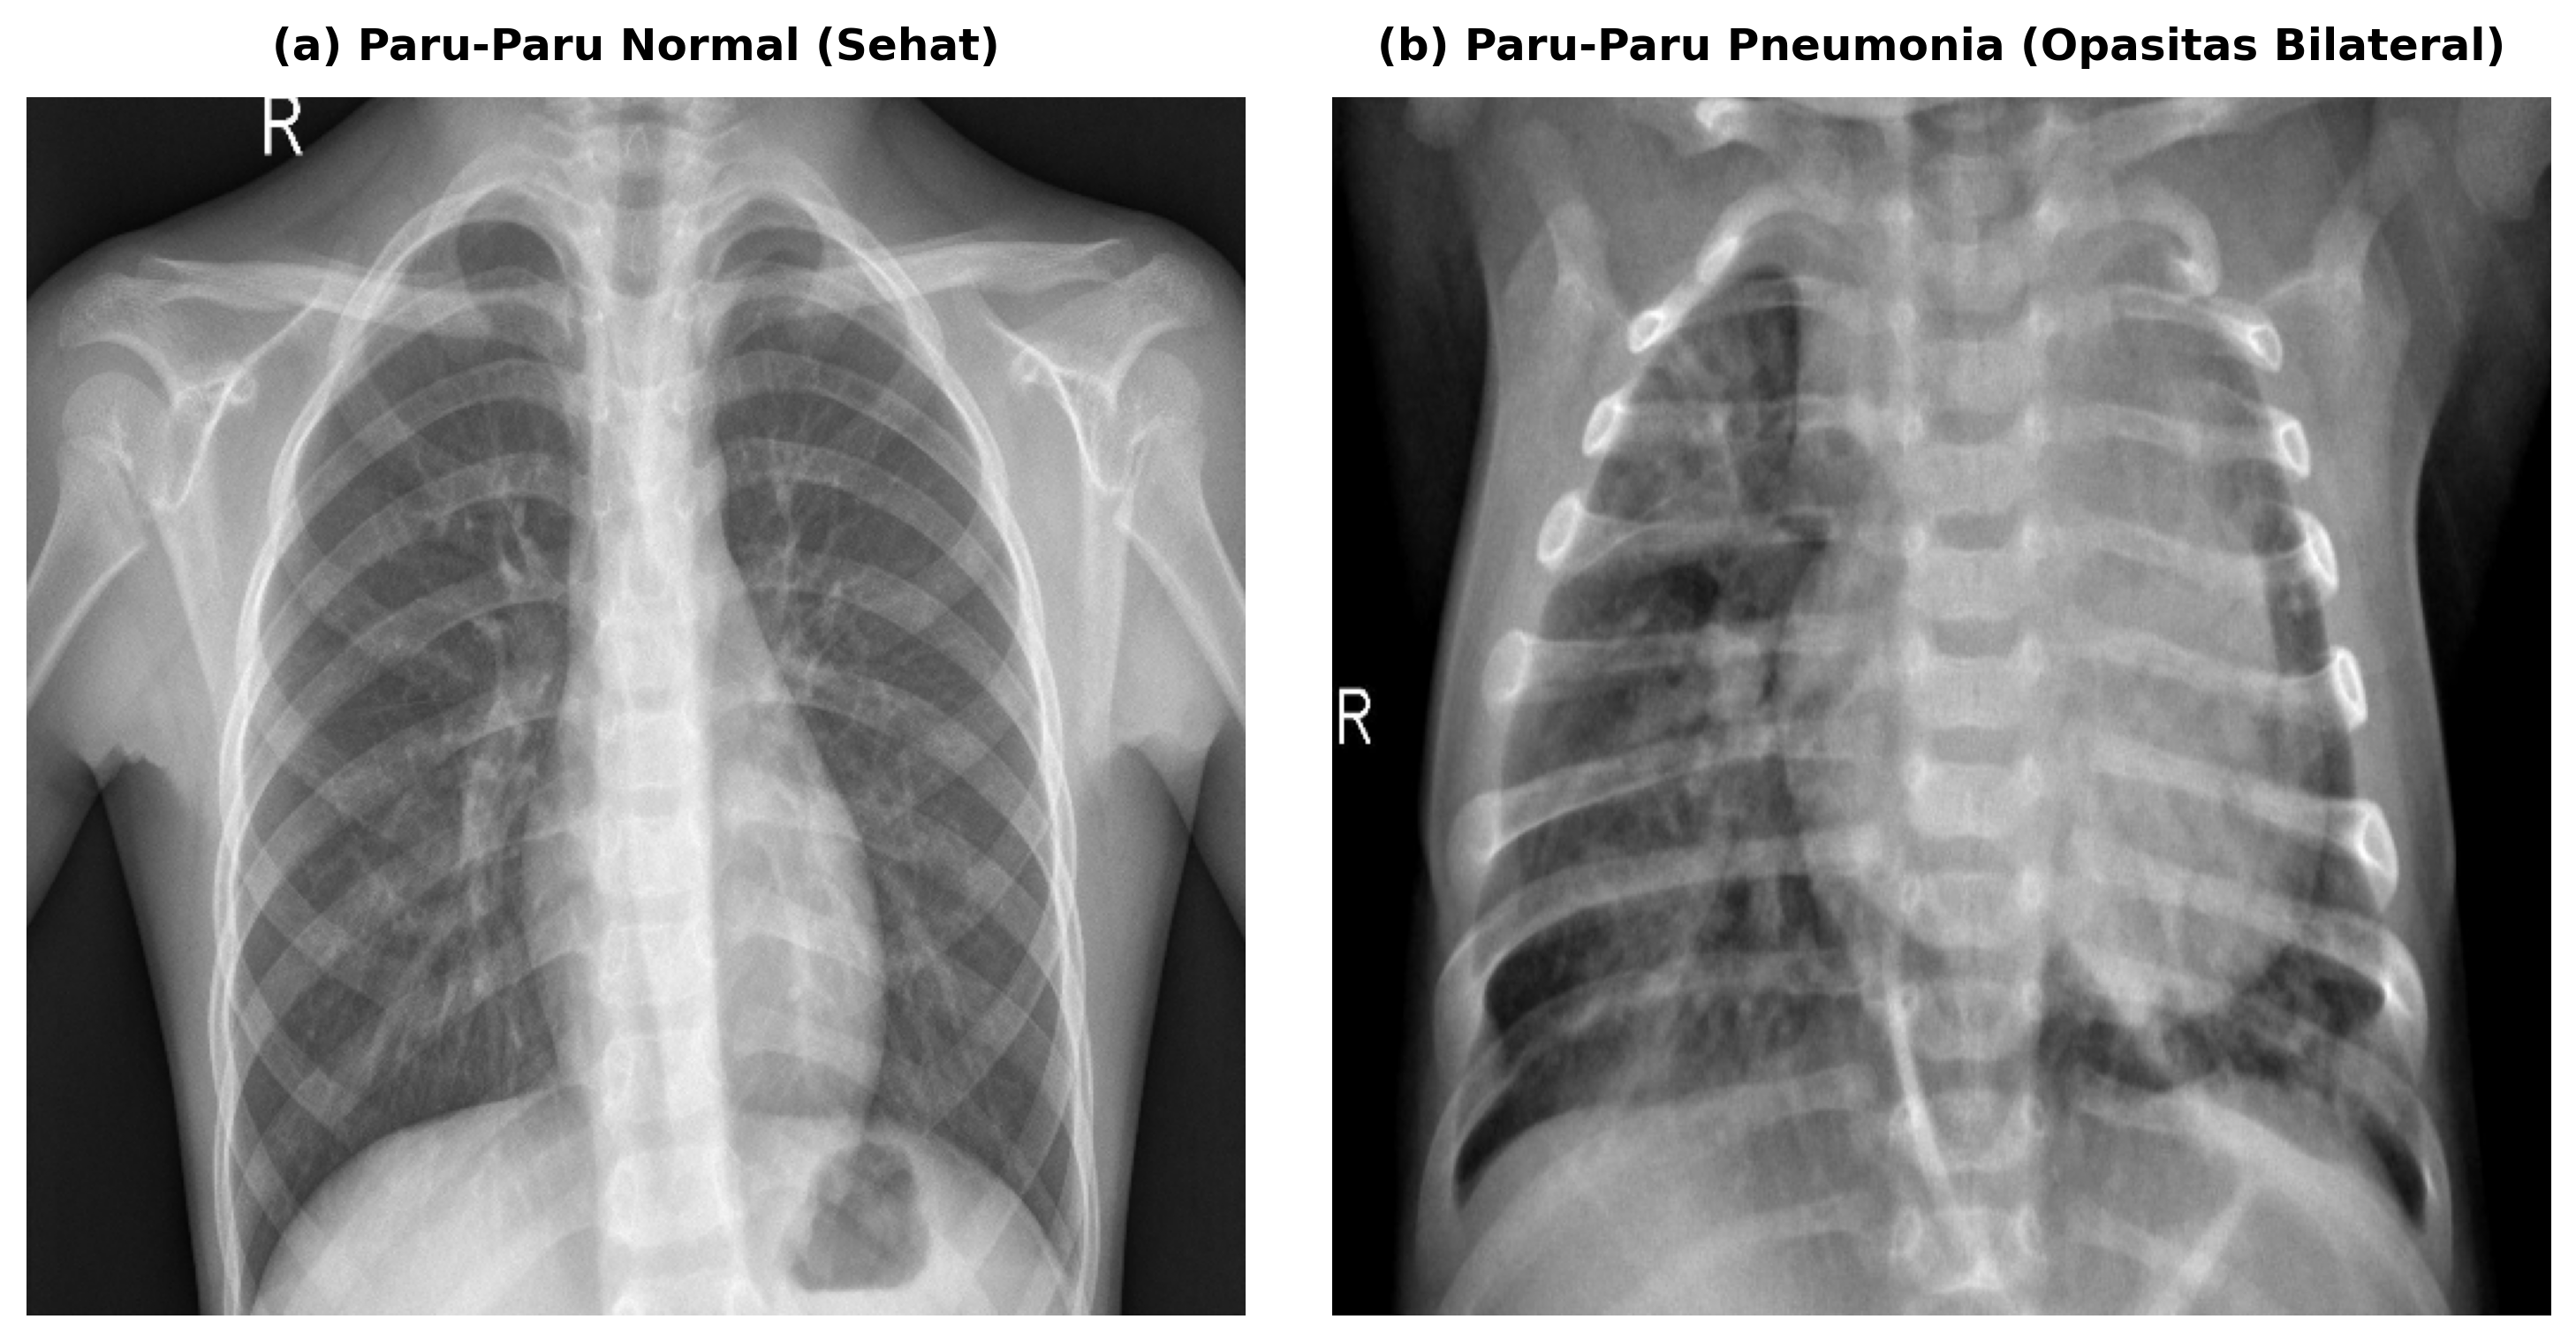
\includegraphics[width=6.67cm, height=2.7cm]{cxr_normal_vs_pneumonia}};

  % Lower Author Info (Left)
  \node[anchor=north west, text=GUBlack, font=\small, align=left]
    at ([xshift=0.4cm, yshift=-5.4cm]current page.north west)
    {\textbf{Nama : Muhammad Hisyam}\\[3pt]
     \textbf{NPM : 51422075}\\[3pt]
     \textbf{Pembimbing : Dr. Tavipia Rumambi, SKom., MMSI.}};

  % Bottom Right Logo (Gunadarma Skripsi)
  \node[anchor=south east, inner sep=12pt]
    at (current page.south east)
    {
\includegraphics[height=1.2cm]{logo_gunadarma}};
  \node[anchor=south east, text=GUMagenta, font=\bfseries\small, inner sep=12pt]
    at ([yshift=1.1cm]current page.south east)
    {SKRIPSI UNIVERSITAS GUNADARMA};
\end{tikzpicture}
\end{frame}
}

% ─── SLIDE 2: LATAR BELAKANG MASALAH ────────────────────────
\begin{frame}{LATAR BELAKANG MASALAH}{Tantangan Diagnostik Pneumonia \& Urgensi Sistem Deteksi Otomatis}
\begin{columns}[T]
  \begin{column}{0.48\textwidth}
    \begin{block}{\footnotesize Beban Klinis \& Keterbatasan Diagnosis Manual}
      \begin{itemize}\scriptsize
        \item \textbf{Mortalitas Tinggi}: Pneumonia merenggut $\sim$\,2,5 juta jiwa global tahun 2019 (WHO), dengan korban terbesar anak di bawah 5 tahun \& lansia.
        \item \textbf{Diagnosis via CXR}: Foto rontgen dada dipilih karena murah \& dosis radiasi rendah dibanding CT Scan, namun rentan salah baca --- terutama di fasilitas minim tenaga ahli.
        \item \textbf{Beban Radiolog}: Kelebihan beban kerja radiolog memperlambat diagnosis, sementara pola lesi pneumonia sering mirip edema atau efusi pleura.
      \end{itemize}
    \end{block}
  \end{column}
  
  \begin{column}{0.48\textwidth}
    \begin{block}{\footnotesize Solusi: Deep Learning \& Explainable AI}
      \begin{itemize}\scriptsize
        \item \textbf{CNN U-Net}: Terbukti mampu segmentasi citra medis piksel-demi-piksel dengan akurasi tinggi.
        \item \textbf{sCSE Attention}: Mekanisme atensi memfokuskan model hanya pada area lesi relevan, mengabaikan bagian tidak penting.
        \item \textbf{EfficientNet-B3 (Transfer Learning)}: Mengatasi keterbatasan data medis --- mempercepat pelatihan \& meningkatkan performa.
        \item \textbf{Grad-CAM \& Gradio Web}: Menjamin transparansi keputusan model \& kemudahan akses bagi tenaga medis.
      \end{itemize}
    \end{block}
  \end{column}
\end{columns}
\vspace{0.05cm}
\begin{alertblock}{\footnotesize Sistem yang Dibangun}
  \scriptsize Penelitian ini membangun sistem \textbf{CDSS} (\textit{Clinical Decision Support System}) berbasis U-Net + sCSE + EfficientNet-B3 mengikuti kerangka CRISP-DM, dilengkapi Grad-CAM dan antarmuka web Gradio yang dapat diakses via internet melalui Cloudflare Tunnel.
\end{alertblock}
\end{frame}

% ─── SLIDE 3: URGENSI SEGMENTASI MEDIS OTOMATIS ──────────────
\begin{frame}{URGENSI SEGMENTASI MEDIS OTOMATIS}{Komparasi Paradigma: Klasifikasi vs. Deteksi Objek vs. Segmentasi Semantik (U-Net)}
\begin{columns}[T]
  \begin{column}{0.31\textwidth}
    \begin{block}{\footnotesize 1. Klasifikasi Biner}
      \scriptsize \textbf{ResNet / VGG}
      \begin{itemize}\scriptsize
        \item \textbf{Output}: Label tunggal (\textit{Pneumonia} vs \textit{Normal}).
        \item \textbf{Keterbatasan}: Tidak memberikan lokasi, batas, maupun luas infeksi.
        \item \textbf{Klinis}: Kurang informatif untuk pemantauan progresivitas.
      \end{itemize}
    \end{block}
  \end{column}

  \begin{column}{0.33\textwidth}
    \begin{block}{\footnotesize 2. Deteksi Objek}
      \scriptsize \textbf{YOLO / Faster R-CNN}
      \begin{itemize}\scriptsize
        \item \textbf{Output}: \textit{Bounding Box} persegi ($(x,y,w,h)$).
        \item \textbf{Keterbatasan}: Lesi ireguler. Box menyertakan banyak jaringan sehat.
        \item \textbf{Klinis}: Kalkulasi rasio keparahan menjadi bias \& tidak akurat.
      \end{itemize}
    \end{block}
  \end{column}

  \begin{column}{0.32\textwidth}
    \begin{block}{\footnotesize 3. Segmentasi U-Net}
      \scriptsize \textbf{U-Net + sCSE (Solusi)}
      \begin{itemize}\scriptsize
        \item \textbf{Output}: Masker biner piksel-demi-piksel (\textit{pixel-wise}).
        \item \textbf{Keunggulan}: Memetakan kontur lesi ireguler secara terperinci.
        \item \textbf{Klinis}: Memungkinkan kalkulasi \textit{Severity Score} (\%).
      \end{itemize}
    \end{block}
  \end{column}
\end{columns}
\end{frame}

% ─── SLIDE 4: RUMUSAN MASALAH & TUJUAN ───────────────────────
\begin{frame}{RUMUSAN MASALAH \& TUJUAN PENELITIAN}{Fokus Utama \& Target Pencapaian Penelitian}
\begin{columns}[T]
  \begin{column}{0.48\textwidth}
    \begin{block}{\footnotesize Rumusan Masalah}
      \begin{enumerate}\scriptsize
        \item Bagaimana membangun dan melatih model deteksi pneumonia menggunakan arsitektur \textbf{U-Net dengan atensi sCSE} dan \textit{encoder} \textbf{EfficientNet-B3} pada dataset RSNA \textit{Pneumonia Detection Challenge}?
        \item Bagaimana pengaruh penggunaan mekanisme atensi \textbf{sCSE} dan pra-pemrosesan segmentasi paru-paru otomatis \textbf{(PSPNet)} terhadap performa model dalam mendeteksi area infeksi pneumonia?
        \item Bagaimana membangun antarmuka aplikasi web yang dapat menampilkan hasil deteksi beserta visualisasi \textbf{Grad-CAM} agar mudah dipahami oleh pengguna?
      \end{enumerate}
    \end{block}
  \end{column}

  \begin{column}{0.48\textwidth}
    \begin{block}{\footnotesize Tujuan Penelitian}
      \begin{enumerate}\scriptsize
        \item Membangun dan melatih model deteksi pneumonia berbasis U-Net dengan atensi sCSE dan \textit{encoder} EfficientNet-B3 pada dataset RSNA \textit{Pneumonia Detection Challenge}.
        \item Mengevaluasi performa model menggunakan metrik segmentasi (\textit{Dice Coefficient}, \textit{Precision}, \textit{Recall}, \textit{Specificity}) serta menganalisis pengaruh sCSE dan PSPNet terhadap hasil deteksi.
        \item Membangun aplikasi web berbasis Gradio yang mengintegrasikan model deteksi dengan visualisasi Grad-CAM agar hasil mudah dipahami pengguna.
      \end{enumerate}
    \end{block}
  \end{column}
\end{columns}
\end{frame}

% ─── SLIDE 5: KERANGKA KERJA CRISP-DM ───────────────────────
\begin{frame}{KERANGKA KERJA CRISP-DM}{Siklus Metodologi Pengembangan Sistem (6 Fase Utama)}
\begin{columns}[c]
  \begin{column}{0.34\textwidth}
    \centering
    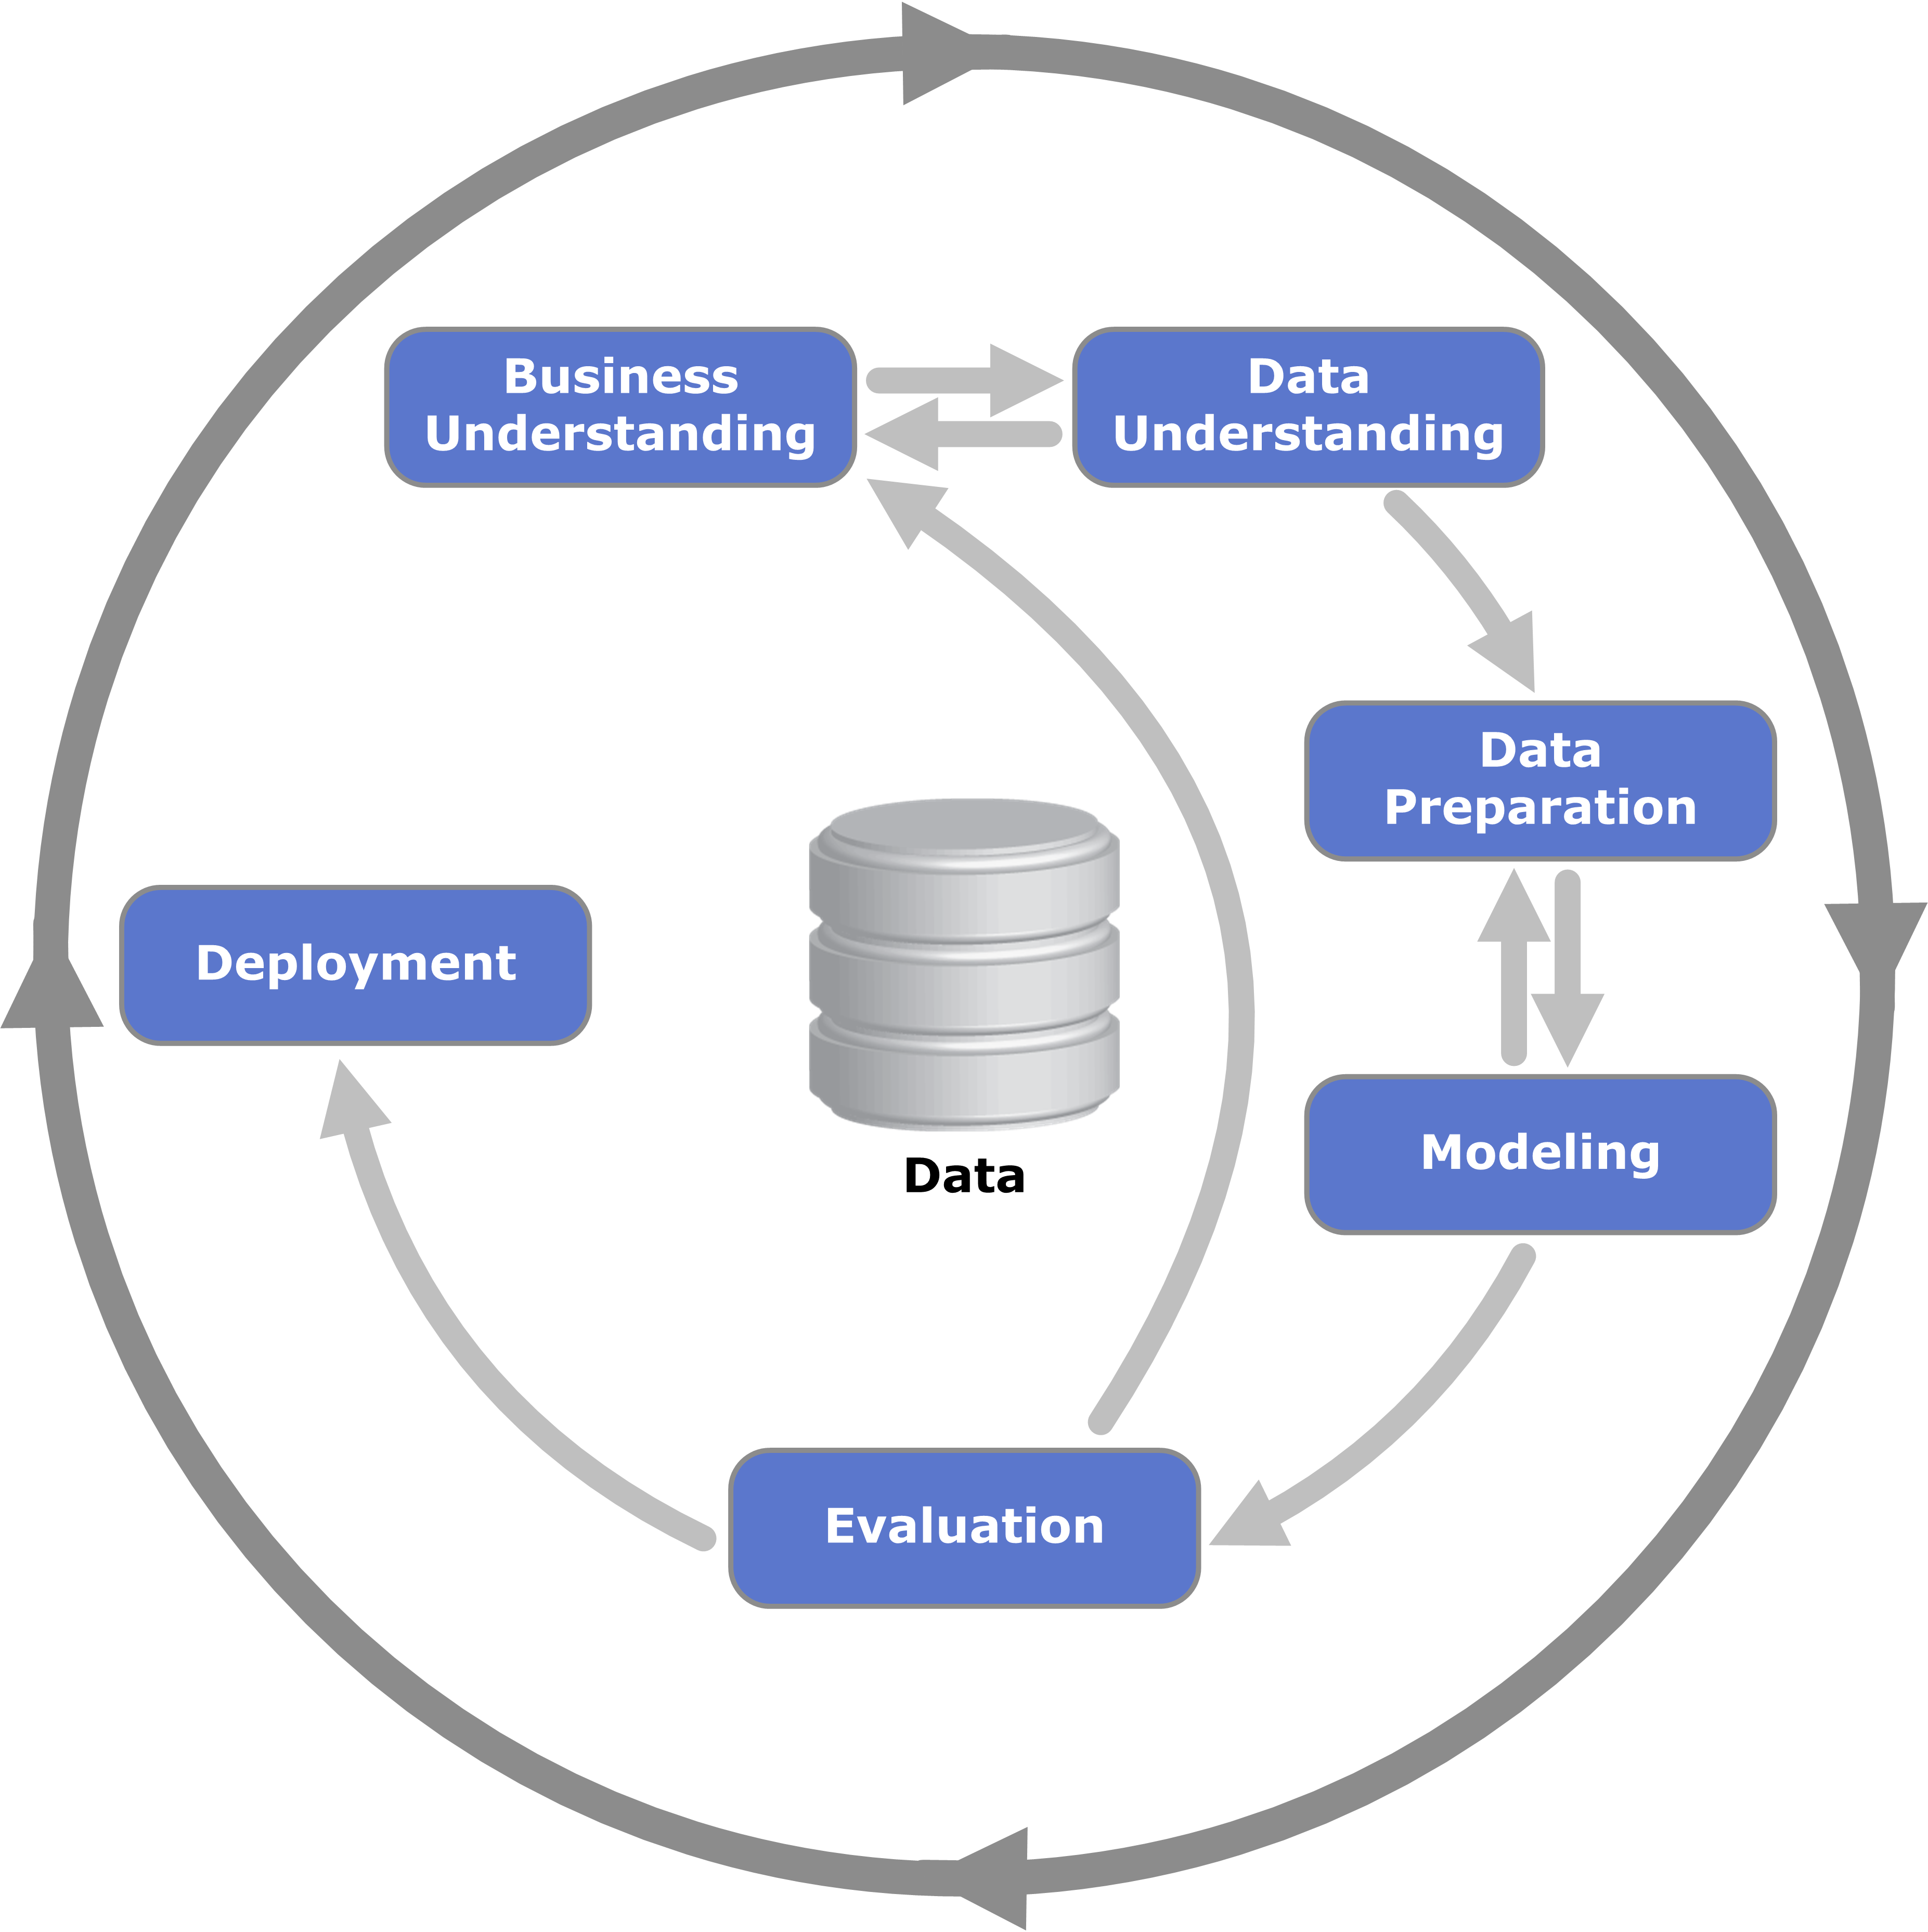
\includegraphics[width=0.85\textwidth]{crisp_dm}
  \end{column}

  \begin{column}{0.62\textwidth}
    \begin{block}{\footnotesize 6 Fase CRISP-DM pada Penelitian Ini}
      \begin{enumerate}\scriptsize
        \item \textbf{Business Understanding}: Kebutuhan CDSS screening awal penunjang keputusan dokter.
        \item \textbf{Data Understanding}: Dataset RSNA Pneumonia (30.227 CXR DICOM), analisis \textit{class imbalance}.
        \item \textbf{Data Preparation}: Konversi DICOM ke PNG 8-bit, CLAHE enhancement, PSPNet Dual Lung Masking, augmentasi data (8 teknik).
        \item \textbf{Modeling}: U-Net + EfficientNet-B3 + sCSE + Unified Focal Loss + pelatihan 2-fase (AdamW, AMP).
        \item \textbf{Evaluation}: Evaluasi kuantitatif (Dice 0,6234, Recall 0,7082) \& validasi visual Grad-CAM.
        \item \textbf{Deployment}: Gradio Web App 4-panel \& Cloudflare Tunnel (\texttt{grad.mhisyam.com}).
      \end{enumerate}
    \end{block}
  \end{column}
\end{columns}
\end{frame}

% ─── SLIDE 6: FLOWCHART PENELITIAN ───────────────────────────
\begin{frame}{FLOWCHART PENELITIAN}{Alur Tahapan Eksperimen \& Pemrosesan Data dari Input hingga Web Deployment}
\begin{columns}[c]
  \begin{column}{0.32\textwidth}
    \centering
    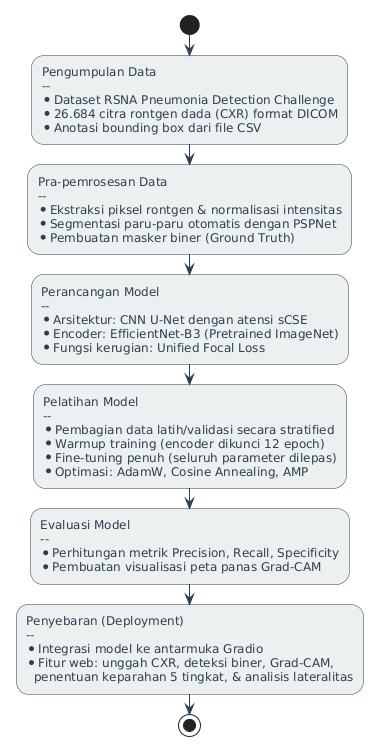
\includegraphics[height=4.5cm]{flowchart_penelitian}
  \end{column}
  
  \begin{column}{0.65\textwidth}
    \begin{block}{\footnotesize Rincian Tahapan Alur Penelitian}
      \begin{itemize}\scriptsize
        \item \textbf{Input Data}: Citra Rontgen Dada DICOM 16-bit dari RSNA Pneumonia Detection Challenge.
        \item \textbf{Preprocessing}: Normalisasi Min-Max, kontras CLAHE, \& segmentasi ROI paru PSPNet.
        \item \textbf{Augmentasi Data}: 8 teknik Albumentations (Rotation, Shift, Brightness, Noise, Dropout).
        \item \textbf{Training U-Net}: Optimizer AdamW, AMP FP16, Unified Focal Loss ($\alpha=0.5, \gamma=2.0$).
        \item \textbf{Evaluasi Model}: Pengujian pada 3.543 citra test set \& Confusion Matrix piksel.
        \item \textbf{XAI \& Web App}: Peta gradien Grad-CAM, kalkulasi Severity Tier, \& Gradio Web deployment.
      \end{itemize}
    \end{block}
  \end{column}
\end{columns}
\end{frame}

% ─── SLIDE 7: DIAGRAM PERANCANGAN SISTEM (UML) ──────────────
\begin{frame}{DIAGRAM PERANCANGAN SISTEM (UML)}{Model Interaksi Pengguna (Use Case) \& Alur Logika Inferensi (Activity Diagram)}
\begin{columns}[c]
  \begin{column}{0.48\textwidth}
    \centering
    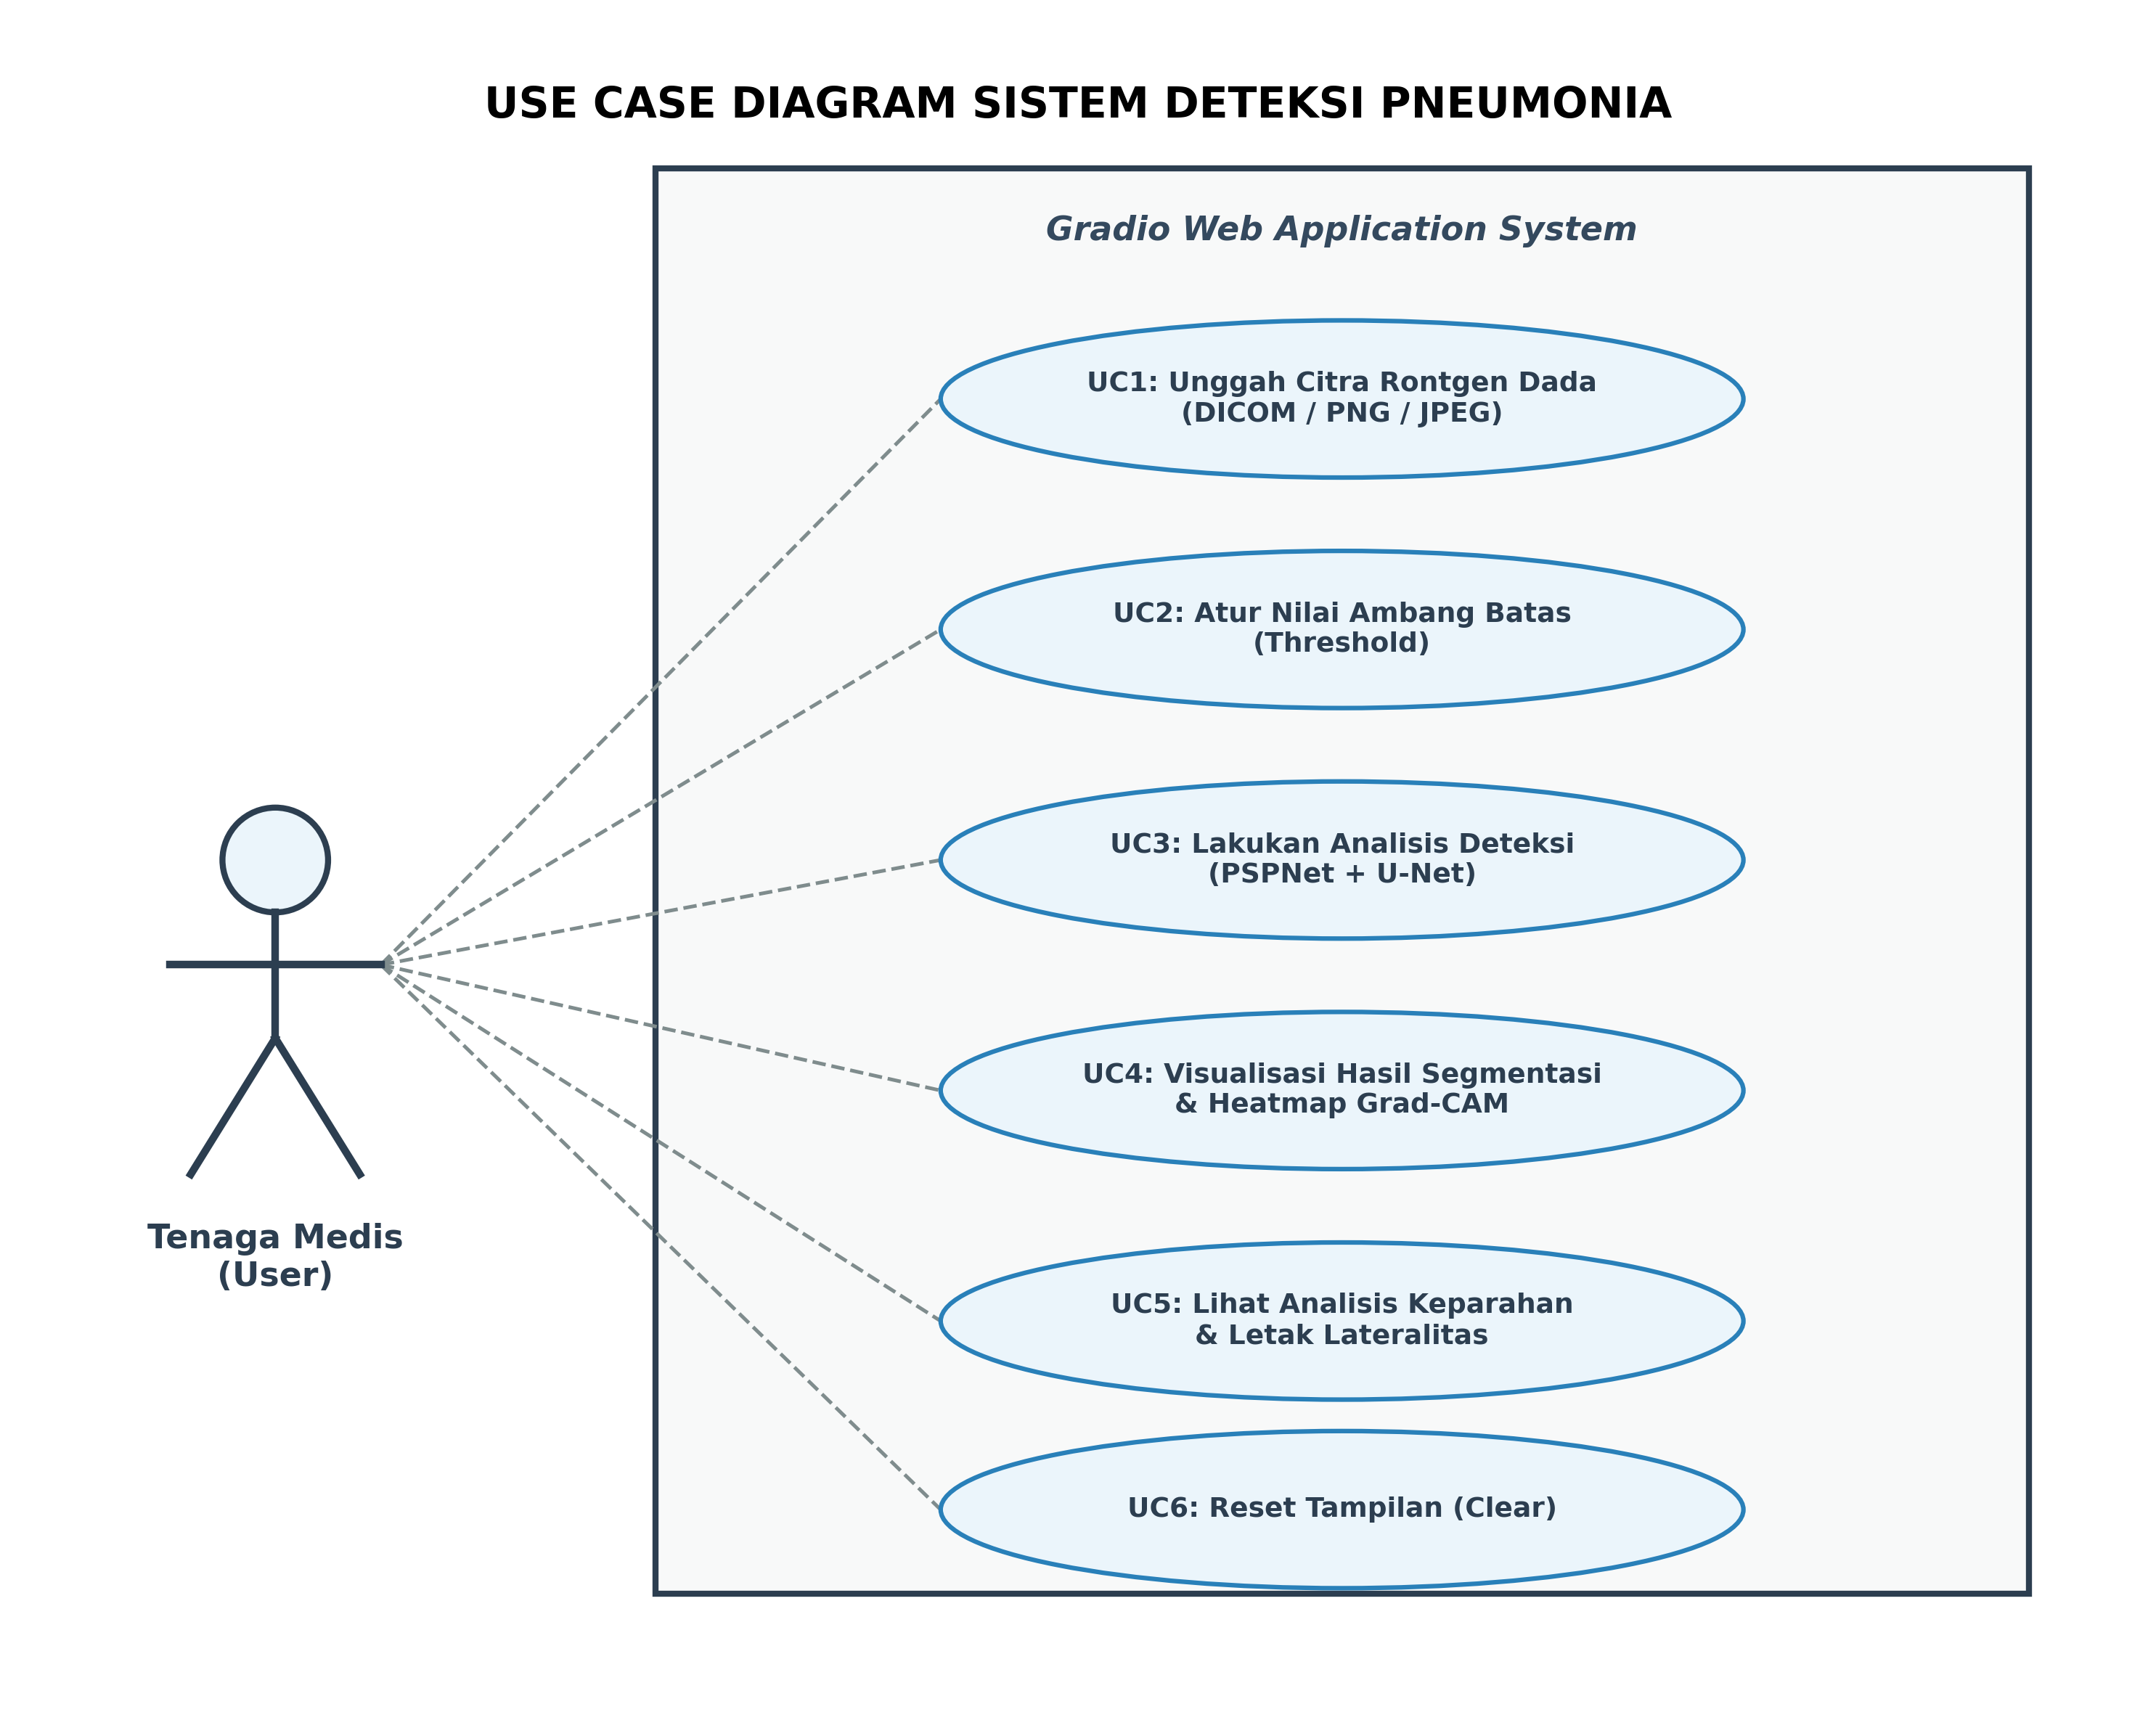
\includegraphics[height=3.2cm, keepaspectratio]{use_case_diagram}
    \begin{block}{\footnotesize Use Case Diagram Aplikasi Web}
      \begin{itemize}\tiny
        \item \textbf{6 Fungsi Utama}: Unggah Citra (DICOM/PNG/JPG), Atur Threshold Slider, Analisis File U-Net, Lihat Overlay \& Grad-CAM, Lihat Laporan Severity, dan Reset.
      \end{itemize}
    \end{block}
  \end{column}

  \begin{column}{0.48\textwidth}
    \centering
    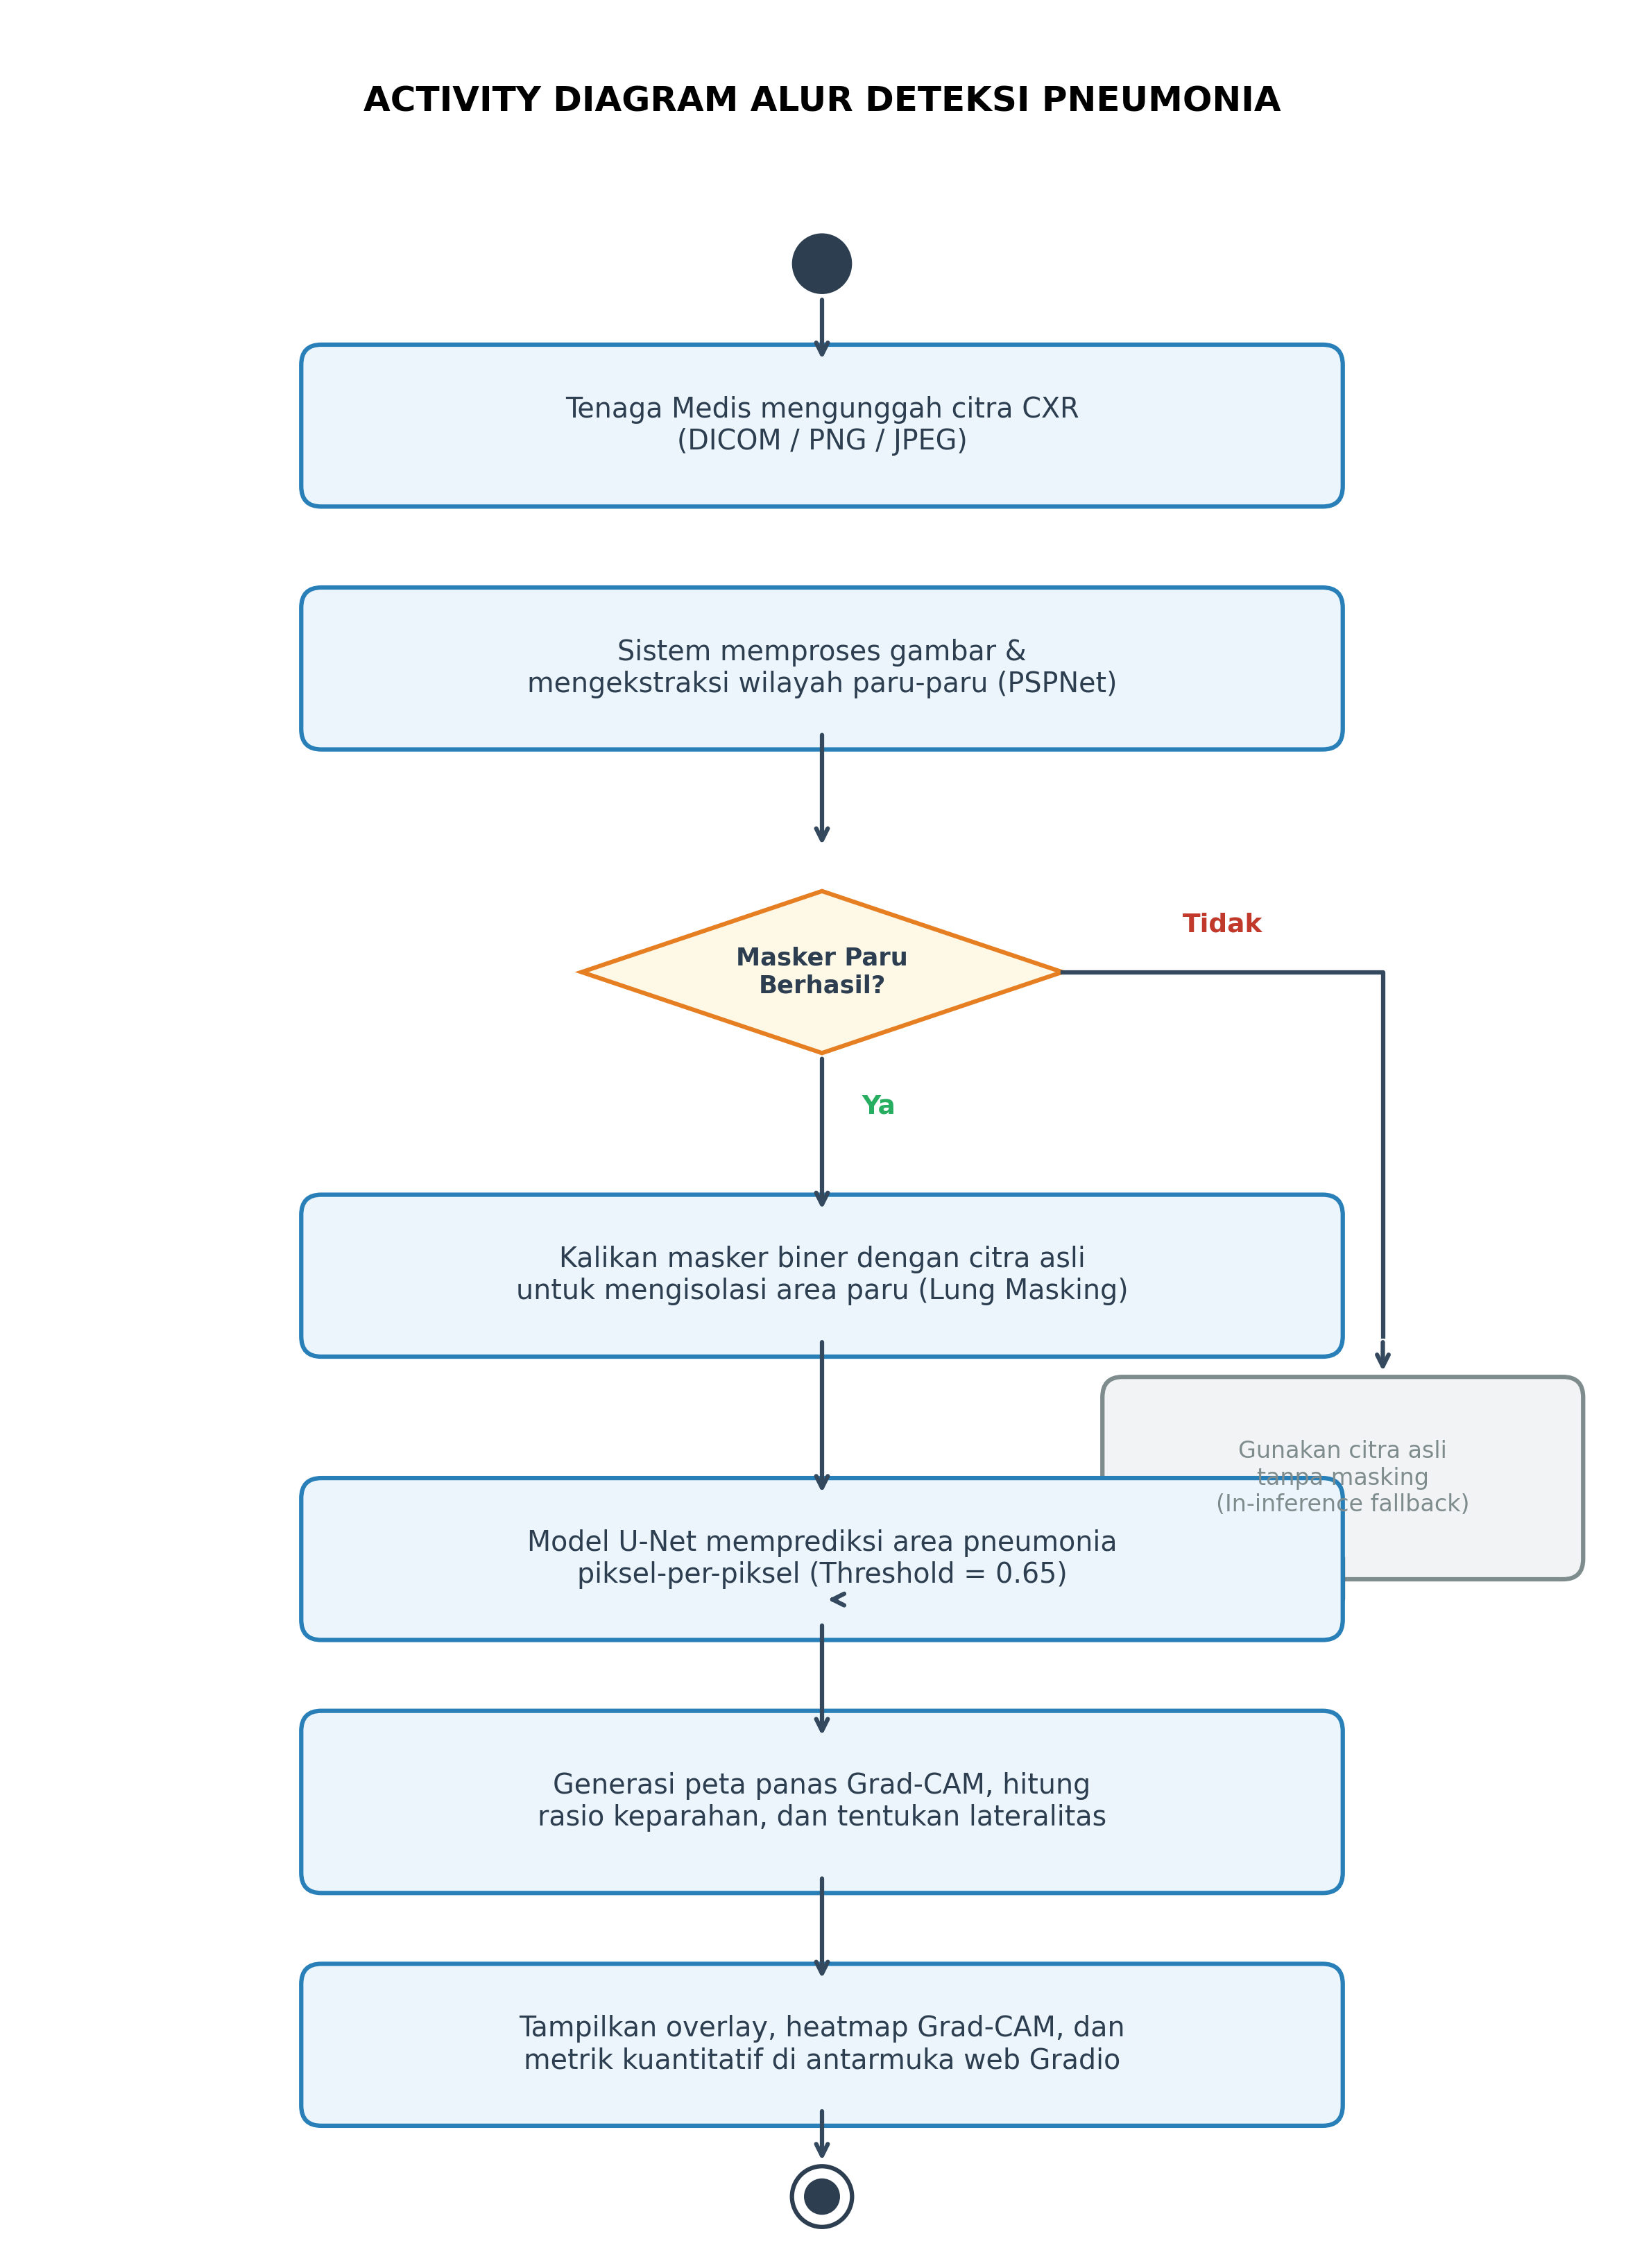
\includegraphics[height=3.2cm, keepaspectratio]{activity_diagram}
    \begin{block}{\footnotesize Activity Diagram Inferensi Medis}
      \begin{itemize}\tiny
        \item \textbf{Alur Logika}: Input Rontgen $\rightarrow$ Preprocessing CLAHE \& PSPNet $\rightarrow$ Inferensi U-Net + sCSE $\rightarrow$ Generasi Heatmap Grad-CAM $\rightarrow$ Output 4-Panel \& Severity Report.
      \end{itemize}
    \end{block}
  \end{column}
\end{columns}
\end{frame}

% ─── SLIDE 8: DATASET & PREPROCESSING ────────────────────────
\begin{frame}{DATASET \& PREPROCESSING PIPELINE}{RSNA Pneumonia Detection Challenge \& Dual Lung Masking}
\begin{columns}[T]
  \begin{column}{0.48\textwidth}
    \begin{block}{\footnotesize Dataset RSNA Pneumonia Challenge}
      \begin{itemize}\scriptsize
        \item \textbf{Total Citra}: 26.684 citra latih DICOM ($1024 \times 1024$).
        \item \textbf{Lung Opacity} (Pneumonia Positif): 6.012 citra (22,5\%).
        \item \textbf{No Lung Opacity / Not Normal}: 7.210 citra (27,1\%).
        \item \textbf{Normal}: 13.462 citra (50,4\%).
        \item \textbf{Patient-Level Split}: Split 80:20 pada tingkat \textit{Patient ID} (mencegah \textit{data leakage}).
      \end{itemize}
    \end{block}
  \end{column}

  \begin{column}{0.48\textwidth}
    \begin{block}{\footnotesize Preprocessing \& Dual Lung Masking}
      \begin{itemize}\scriptsize
        \item \textbf{16-bit ke 8-bit}: Normalisasi Min-Max $[0, 255]$ \& resize $512 \times 512$.
        \item \textbf{CLAHE}: Peningkatan kontras lokal (\texttt{clip\_limit=2.0}, tile $8 \times 8$).
        \item \textbf{PSPNet Dual Lung Masking}: Memotong ROI paru kiri \& kanan, mengeliminasi teks DICOM, kabel EKG, \& penanda L/R.
        \item \textbf{8 Augmentasi}: Horizontal Flip, Shift-Scale-Rotate, Gamma, Noise, Coarse/Grid Dropout.
      \end{itemize}
    \end{block}
  \end{column}
\end{columns}
\end{frame}

% ─── SLIDE 8: KONSEP DASAR CONVOLUTIONAL NEURAL NETWORK (CNN) ───
\begin{frame}{KONSEP DASAR CONVOLUTIONAL NEURAL NETWORK (CNN)}{Prinsip Ekstraksi Fitur Citra: Operasi Konvolusi, Fungsi Aktivasi, \& Pooling}
\begin{columns}[c]
  \begin{column}{0.48\textwidth}
    \begin{block}{\footnotesize Komponen Utama Arsitektur CNN}
      \begin{itemize}\scriptsize
        \item \textbf{Operasi Konvolusi ($Y = f(W * X + b)$)}: Perkalian kernel filter terhadap piksel citra untuk mengekstrak fitur spasial (tepi, tekstur, opasitas).
        \item \textbf{Fungsi Aktivasi (ReLU / Swish)}: Transformasi non-linear ($\max(0, x)$) agar jaring mempelajari pola lesi ireguler yang kompleks.
        \item \textbf{Pooling Layer (Max/Average)}: Reduksi dimensi spasial (\textit{downsampling}) untuk efisiensi komputasi \& ketahanan variasi posisi.
        \item \textbf{Feature Maps Hirarkis}: Ekstraksi dari fitur tingkat rendah (\textit{edges}) hingga tingkat tinggi (\textit{infiltrat pneumonia}).
      \end{itemize}
    \end{block}
  \end{column}

  \begin{column}{0.48\textwidth}
    \centering
    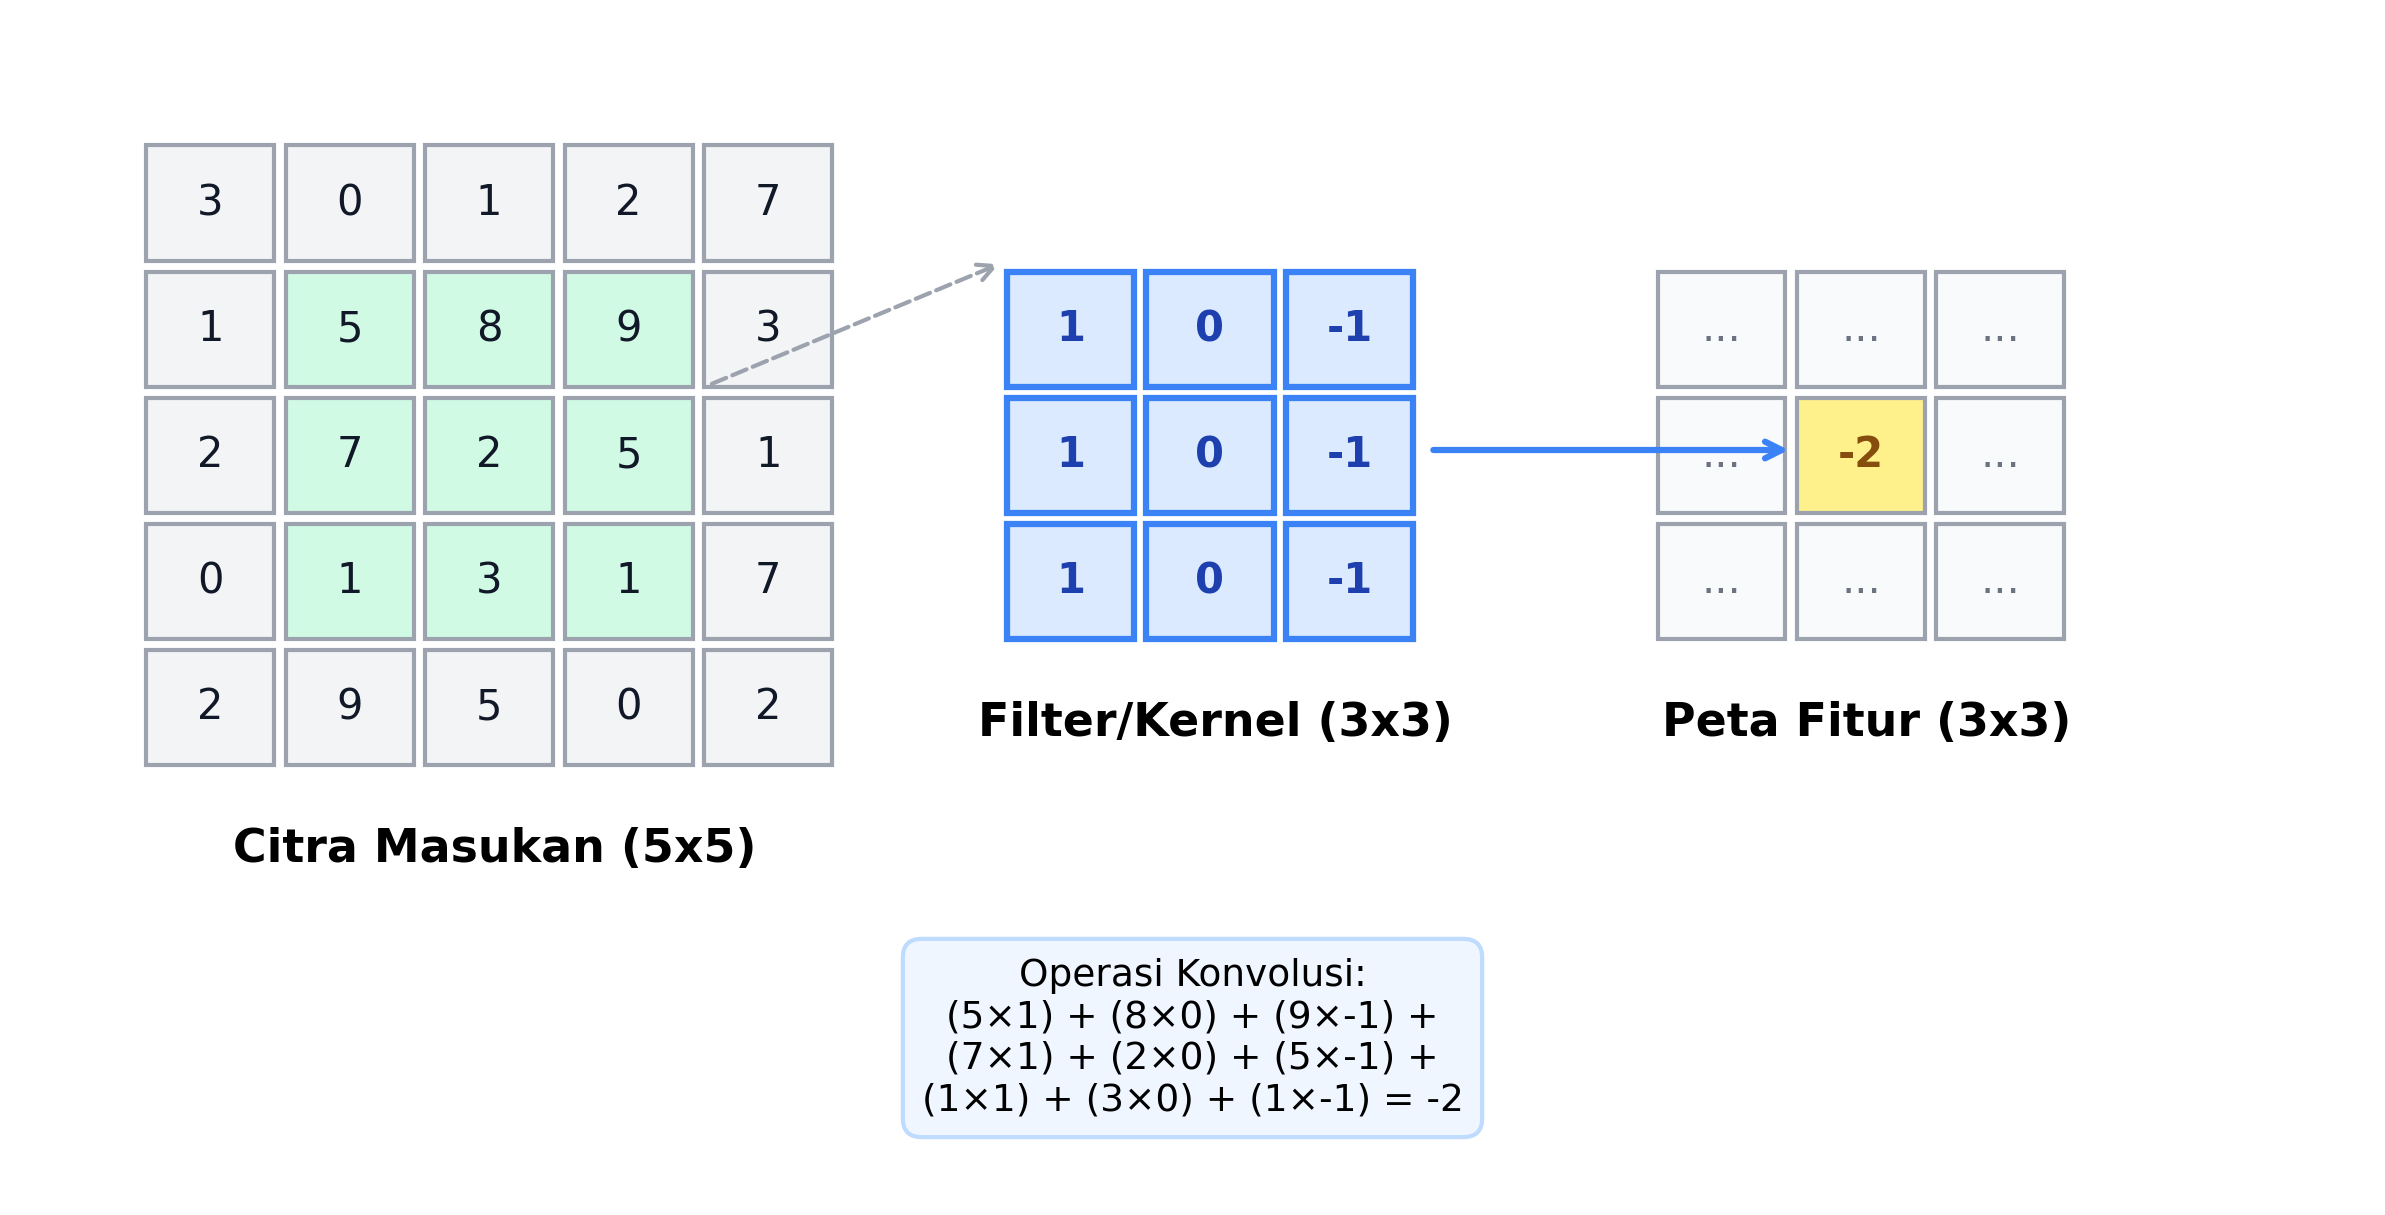
\includegraphics[width=0.88\textwidth, height=2.9cm, keepaspectratio]{operasi_konvolusi}
    \begin{block}{\footnotesize Keunggulan CNN pada Segmentasi Medis}
      \begin{itemize}\tiny
        \item \textbf{Parameter Sharing}: Penggunaan ulang bobot kernel di seluruh piksel citra, meminimalkan risiko \textit{overfitting}.
        \item \textbf{Spatial Hierarchy}: Mempertahankan relasi spasial antar-piksel tetangga pada organ paru.
        \item \textbf{Pretrained Backbone}: Menjadi fondasi \textit{Feature Extractor} pada arsitektur U-Net (EfficientNet-B3).
      \end{itemize}
    \end{block}
  \end{column}
\end{columns}
\end{frame}

% ─── SLIDE 9: ARSITEKTUR U-NET & FORMULA ─────────────────────
\begin{frame}{ARSITEKTUR U-NET \& FORMULASI MATEMATIKA}{U-Net + EfficientNet-B3 Backbone + sCSE Attention Gate + Unified Focal Loss}
\begin{columns}[T]
  \begin{column}{0.50\textwidth}
    \centering
    \scalebox{0.65}{
    \begin{tikzpicture}[node distance=0.75cm, auto, >=Stealth]
      \tikzstyle{enc} = [rectangle, draw=GUMagenta, fill=GULightPink!50, thick, minimum width=1.5cm, minimum height=0.55cm, font=\tiny\bfseries]
      \tikzstyle{dec} = [rectangle, draw=GUPurple, fill=GULightPink!90, thick, minimum width=1.5cm, minimum height=0.55cm, font=\tiny\bfseries]
      
      % Input
      \node (in) [font=\tiny\bfseries] {Input $512^2\times 3$};
      % Encoder
      \node (e1) [enc, below of=in] {Enc 1 (40ch)};
      \node (e2) [enc, below of=e1, yshift=-0.1cm] {Enc 2 (48ch)};
      \node (e3) [enc, below of=e2, yshift=-0.1cm] {Enc 3 (136ch)};
      \node (b)  [enc, draw=red, fill=red!20, below of=e3, yshift=-0.1cm] {Bottleneck (1536ch)};
      
      % Decoder
      \node (d3) [dec, right of=e3, xshift=2.2cm] {Dec 3 + sCSE};
      \node (d2) [dec, right of=e2, xshift=2.2cm] {Dec 2 + sCSE};
      \node (d1) [dec, right of=e1, xshift=2.2cm] {Dec 1 + sCSE};
      \node (out) [font=\tiny\bfseries, right of=in, xshift=3.7cm] {Mask $512^2\times 1$};
      
      % Connections
      \draw[->, thick] (in) -- (e1);
      \draw[->, thick] (e1) -- (e2);
      \draw[->, thick] (e2) -- (e3);
      \draw[->, thick] (e3) -- (b);
      \draw[->, thick] (b) |- (d3);
      \draw[->, thick] (d3) -- (d2);
      \draw[->, thick] (d2) -- (d1);
      \draw[->, thick] (d1) -- (out);
      
      % Skip Connections with sCSE
      \draw[->, dashed, color=GUMagenta, thick] (e3) -- node[above, font=\tiny] {Skip + sCSE} (d3);
      \draw[->, dashed, color=GUMagenta, thick] (e2) -- node[above, font=\tiny] {Skip + sCSE} (d2);
      \draw[->, dashed, color=GUMagenta, thick] (e1) -- node[above, font=\tiny] {Skip + sCSE} (d1);
    \end{tikzpicture}
    }
  \end{column}

  \begin{column}{0.48\textwidth}
    \begin{block}{\footnotesize Alur Kerja Arsitektur U-Net}
      \begin{itemize}\tiny
        \item \textbf{Encoder (Contracting Path)}: EfficientNet-B3 \textit{pretrained} ImageNet mengekstraksi fitur semantik bertingkat dari citra rontgen ($512 \times 512$).
        \item \textbf{Decoder (Expanding Path)}: Melakukan \textit{upsampling} resolusi spasial secara bertahap untuk merekonstruksi piksel masker segmentasi lesi.
        \item \textbf{Skip Connections}: Mengalirkan detail kontur spasial organ langsung dari \textit{encoder} ke \textit{decoder} agar batas organ tidak hilang.
      \end{itemize}
    \end{block}

    \begin{block}{\footnotesize Inovasi Atensi sCSE \& Loss Function}
      \begin{itemize}\tiny
        \item \textbf{Atensi sCSE (Spatial \& Channel)}: Menyaring lokasi lesi (\textit{spasial}) \& tekstur opasitas (\textit{kanal}) untuk menajamkan kontras fitur lesi.
        \item \textbf{Unified Focal Loss}: Memfokuskan pelatihan pada piksel sulit (\textit{hard pixels}) \& menekan angka \textit{False Positives}.
      \end{itemize}
    \end{block}
  \end{column}
\end{columns}
\end{frame}

% ─── SLIDE 10: HASIL EVALUASI KUANTITATIF & CONFUSION MATRIX ─
\begin{frame}[shrink=5]{HASIL EVALUASI KUANTITATIF \& CONFUSION MATRIX}{Evaluasi Performa Segmentasi pada Data Validasi (350.224.384 Total Piksel)}
\begin{columns}[T]
  \begin{column}{0.44\textwidth}
    \begin{block}{\footnotesize Metrik Utama Performa (KPI $\ge 0,60$)}
      \begin{itemize}\scriptsize
        \item \textbf{Dice Coefficient}: \textbf{0.6234} (62,34\%)
        \item \textbf{Precision}: \textbf{0.6868} (68,68\%)
        \item \textbf{Recall (Sensitivitas)}: \textbf{0.7082} (70,82\%)
        \item \textbf{Specificity}: \textbf{0.9781} (97,81\%)
        \item \textbf{Validation Loss}: \textbf{0.2755} (Epoch 46)
      \end{itemize}
    \end{block}
  \end{column}

  \begin{column}{0.53\textwidth}
    \begin{block}{\footnotesize Confusion Matrix Piksel}
      \centering
      \tiny
      \begin{tabular}{lcc}
        \toprule
        & \textbf{Pred. Normal} & \textbf{Pred. Pneumonia} \\
        \midrule
        \textbf{Act. Normal} & \textbf{TN=312.284.691} (97,81\%) & \textbf{FP=7.198.145} (2,19\%) \\
        \textbf{Act. Pneumonia} & \textbf{FN=9.995.562} (29,18\%) & \textbf{TP=20.745.986} (70,82\%) \\
        \bottomrule
      \end{tabular}
    \end{block}
    \begin{exampleblock}{\footnotesize Signifikansi Klinis}
      \scriptsize Recall 70,82\% meminimalkan risiko \textit{false negative} medis, sementara Specificity 97,81\% mencegah \textit{false alarm} berlebih.
    \end{exampleblock}
  \end{column}
\end{columns}
\end{frame}

% ─── SLIDE 10: PERBANDINGAN BASELINE & ABLATION STUDY ───────
\begin{frame}{PERBANDINGAN BASELINE \& ABLATION STUDY}{Analisis Kontribusi Inkremental Komponen Model (+14,1\% Dice Total Gain)}
\centering
\scriptsize
\begin{tabular}{lcccc}
  \toprule
  \textbf{Konfigurasi Komponen Model} & \textbf{Dice} & \textbf{Recall} & \textbf{Precision} & \textbf{$\Delta$ Dice} \\
  \midrule
  Baseline U-Net (Tanpa Pretrain) & 0.4820 & 0.5310 & 0.5240 & — \\
  + EfficientNet-B3 Pretrained ImageNet & 0.5410 & 0.6070 & 0.5730 & +5,9\% \\
  + sCSE Attention Gate & 0.5890 & 0.6620 & 0.6280 & +4,8\% \\
  + Unified Focal Loss ($\alpha=0.5, \gamma=2.0$) & 0.6080 & 0.6940 & 0.6610 & +1,9\% \\
  \rowcolor{GULightPink!50}
  \textbf{+ CLAHE \& Augmentasi Data (Model Final)} & \textbf{0.6234} & \textbf{0.7082} & \textbf{0.6868} & \textbf{+1,5\%} \\
  \bottomrule
\end{tabular}

\vspace{0.15cm}
\begin{block}{\footnotesize Key Takeaways Ablation Study}
  \begin{itemize}\scriptsize
    \item Pemanfaatan bobot ImageNet pada encoder EfficientNet-B3 memberikan lonjakan terbesar (\textbf{+5,9\% Dice}).
    \item Atensi sCSE memperjelas batas lesi \& menyaring fitur relevan pada skip connections (\textbf{+4,8\% Dice}).
    \item Total peningkatan kumulatif Dice Score mencapai \textbf{+14,1\%} dibanding U-Net baseline standar (0.4820 ke 0.6234).
  \end{itemize}
\end{block}
\end{frame}

% ─── SLIDE 11: VISUALISASI SEGMENTASI KLINIS ────────────────
\begin{frame}{VISUALISASI SEGMENTASI KLINIS}{Evaluasi 4 Sampel Kasus Medis (4 Kolom: CXR, PSPNet Masking, Overlay, Heatmap)}
\centering
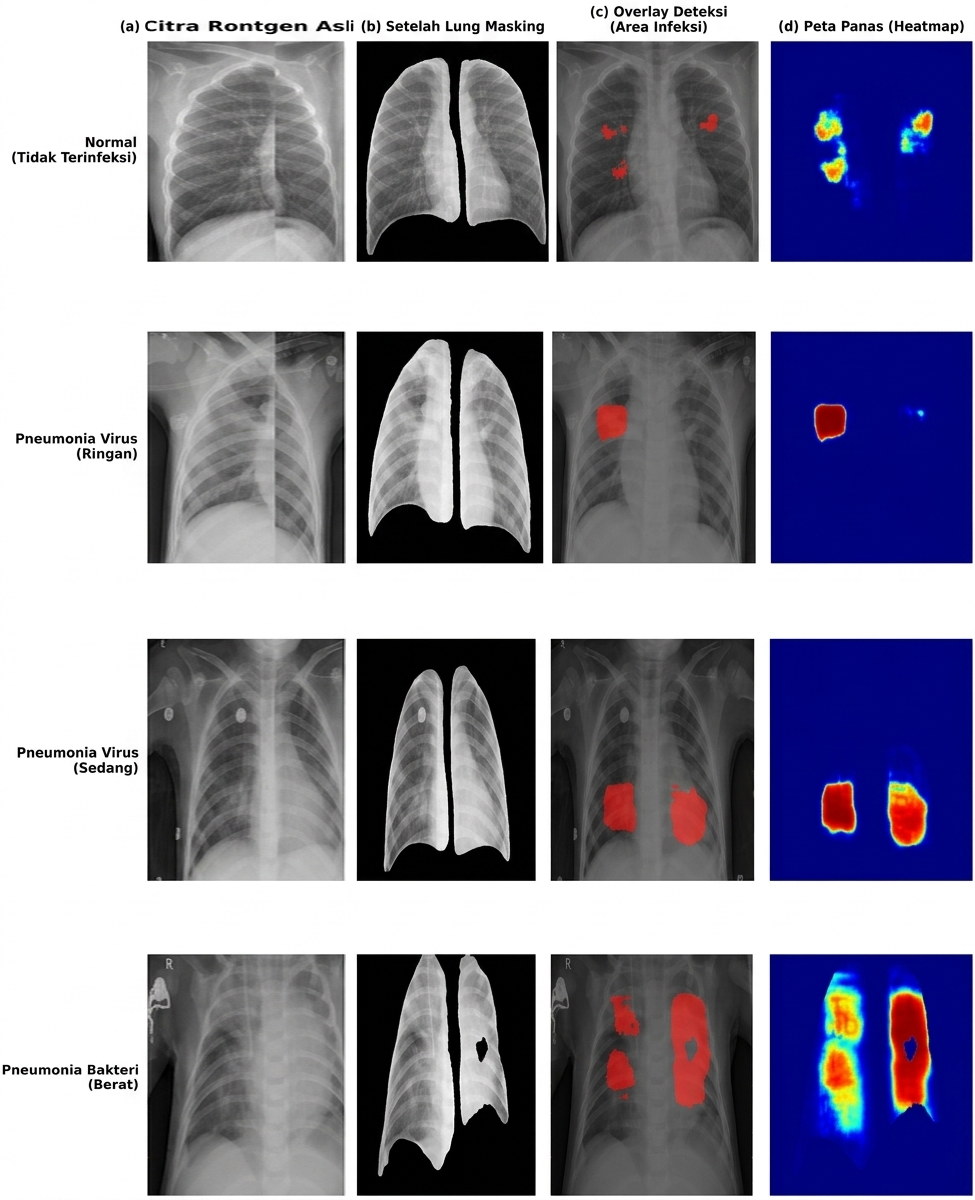
\includegraphics[width=0.72\textwidth, height=2.8cm, keepaspectratio]{hasil_segmentasi_visual}

\vspace{0.05cm}
\begin{columns}[T]
  \begin{column}{0.24\textwidth}
    \centering \tiny \textbf{(a) Citra CXR Asli}\\
    Rontgen mentah pasien
  \end{column}
  \begin{column}{0.24\textwidth}
    \centering \tiny \textbf{(b) PSPNet Lung Mask}\\
    Hasil pemotongan ROI organ
  \end{column}
  \begin{column}{0.24\textwidth}
    \centering \tiny \textbf{(c) Overlay Prediction}\\
    Masker U-Net (Arsir Merah)
  \end{column}
  \begin{column}{0.24\textwidth}
    \centering \tiny \textbf{(d) Grad-CAM Heatmap}\\
    Peta aktivasi JET colormap
  \end{column}
\end{columns}
\end{frame}

% ─── SLIDE 12: EXPLAINABLE AI (GRAD-CAM & SEVERITY) ─────────
\begin{frame}{EXPLAINABLE AI (XAI) \& SEVERITY SCORING}{Interpretasi Medis Heatmap Grad-CAM \& Tingkat Keparahan Infeksi}
\begin{columns}[T]
  \begin{column}{0.50\textwidth}
    \begin{block}{\footnotesize JET Colormap Spectrum Table}
      \centering
      \tiny
      \begin{tabular}{lcl}
        \toprule
        \textbf{Warna} & \textbf{Probabilitas} & \textbf{Interpretasi Klinis} \\
        \midrule
        \rowcolor{red!20} \textbf{Merah} & $0,8 - 1,0$ & Pusat lesi infeksi / gradien dominan \\
        \rowcolor{yellow!20} \textbf{Kuning} & $0,6 - 0,8$ & Aktivasi tinggi / margin lesi transisi \\
        \rowcolor{green!20} \textbf{Hijau} & $0,3 - 0,6$ & Aktivasi sedang / perilesional \\
        \rowcolor{blue!10} \textbf{Biru} & $0,0 - 0,3$ & Jaringan paru sehat / background \\
        \bottomrule
      \end{tabular}
    \end{block}
  \end{column}

  \begin{column}{0.46\textwidth}
    \begin{block}{\footnotesize 5-Tier Severity Scoring System}
      \begin{itemize}\tiny
        \item \textbf{Level 0 (Normal)}: $0\%$ rasio infeksi.
        \item \textbf{Level 1 (Mild)}: $\le 5\%$ luas organ paru.
        \item \textbf{Level 2 (Moderate)}: $5\% - 15\%$ luas organ paru.
        \item \textbf{Level 3 (Severe)}: $15\% - 30\%$ luas organ paru.
        \item \textbf{Level 4 (Critical)}: $> 30\%$ luas organ paru.
        \item \textbf{Lateralitas}: Dextra, Sinistra, Bilateral.
      \end{itemize}
    \end{block}
  \end{column}
\end{columns}
\end{frame}

% ─── SLIDE 13: TAMPILAN WEBSITE & CLOUDFLARE TUNNEL ─────────
\begin{frame}{TAMPILAN WEBSITE \& CLOUDFLARE TUNNEL DEPLOYMENT}{Antarmuka Web Gradio Interaktif \& Akses Publik Terenkripsi HTTPS}
\begin{columns}[c]
  \begin{column}{0.48\textwidth}
    \centering
    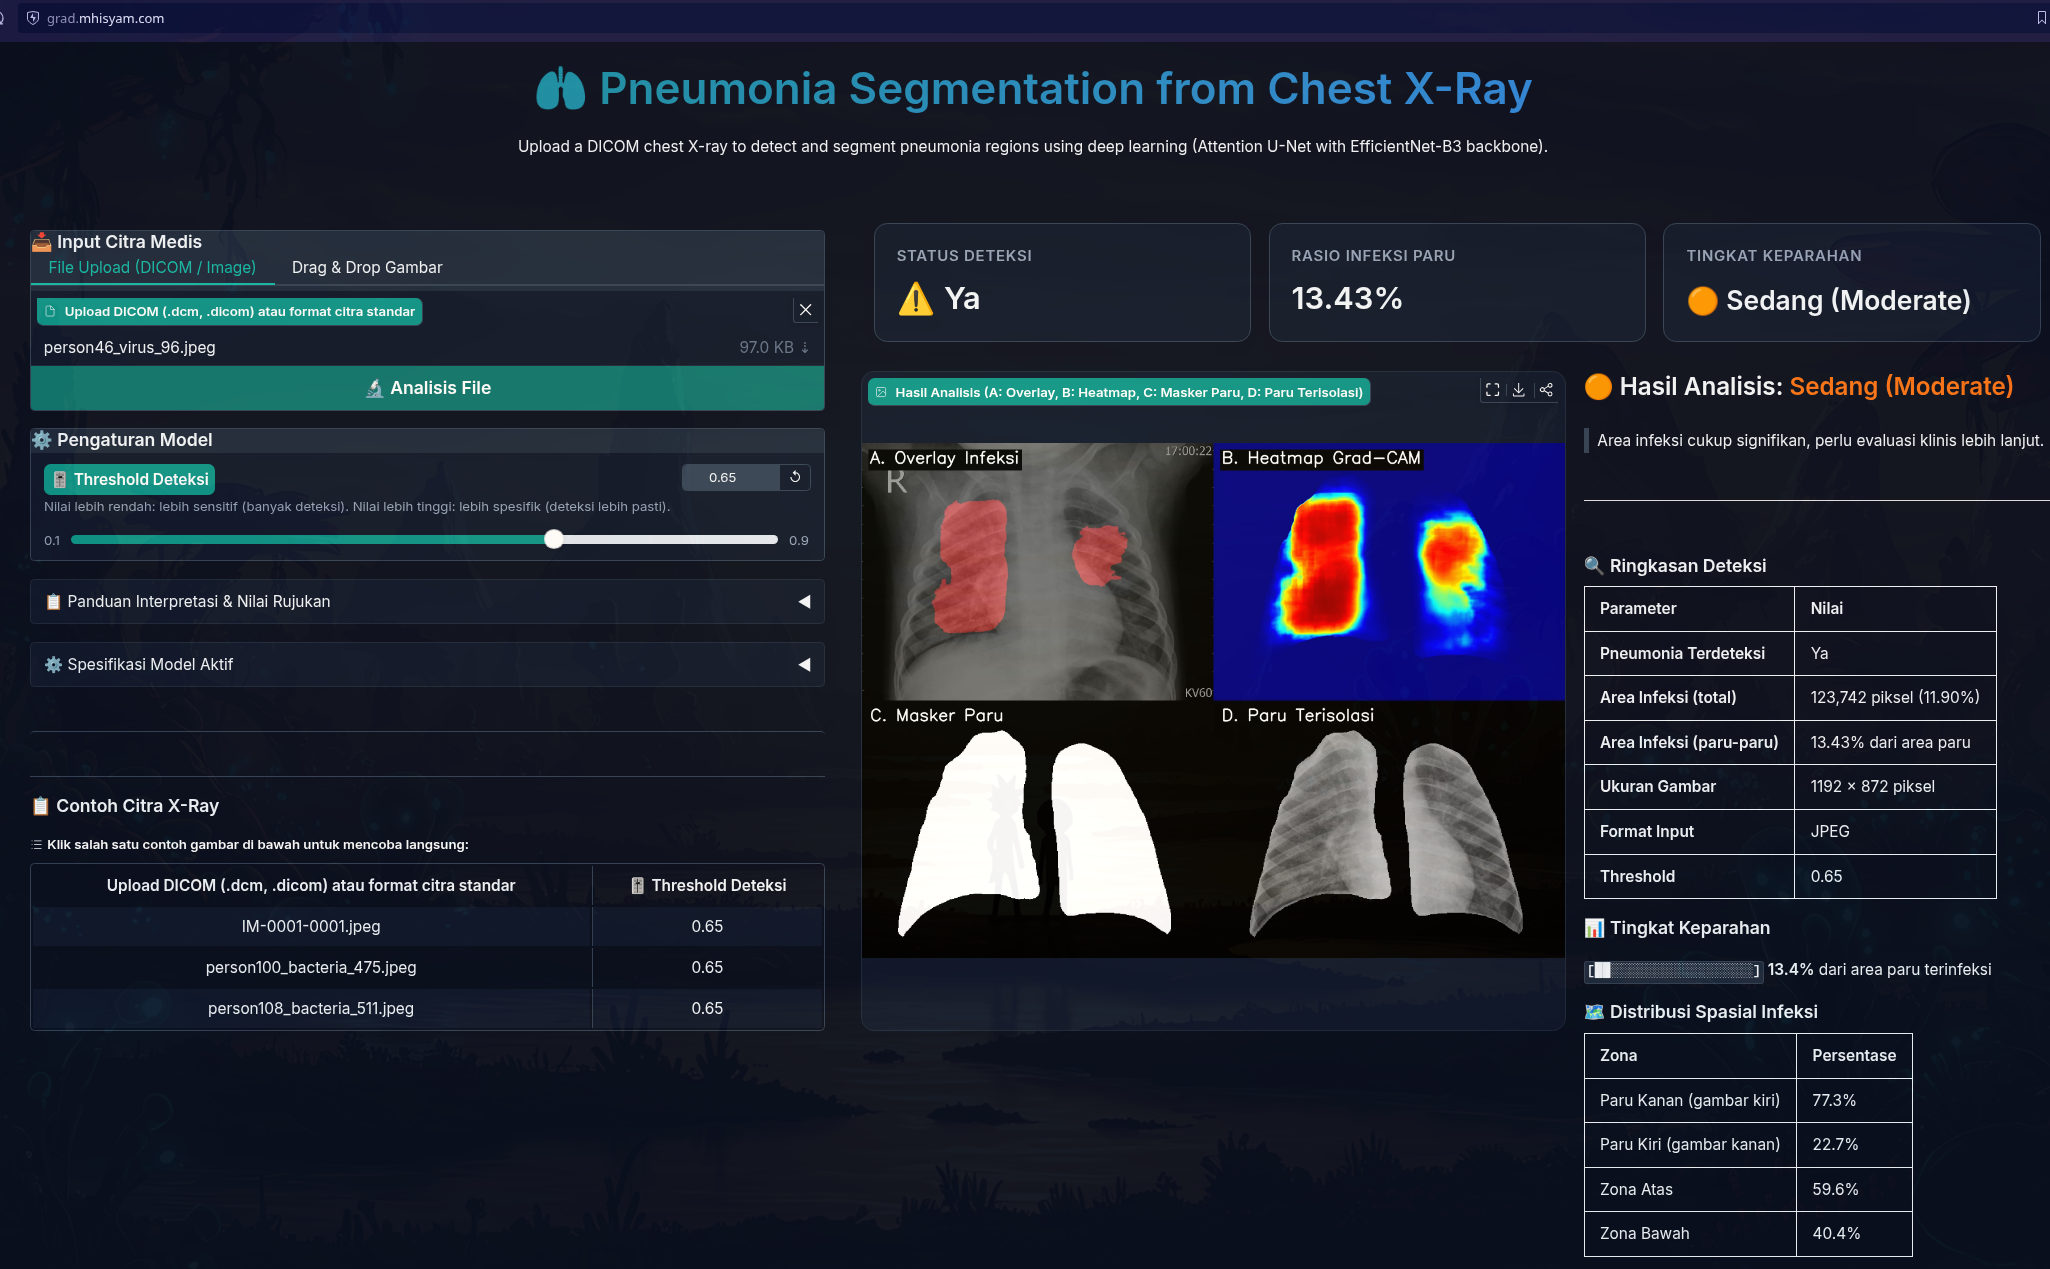
\includegraphics[width=0.78\textwidth]{implementasi_web_gradio}
    \begin{block}{\footnotesize Fitur Gradio Web App}
      \begin{itemize}\tiny
        \item Dual Input (DICOM / PNG / JPG).
        \item Interactive Threshold Slider ($0.1 - 0.9$).
        \item Visual 4-Panel Output \& Laporan Severity.
      \end{itemize}
    \end{block}
  \end{column}

  \begin{column}{0.48\textwidth}
    \centering
    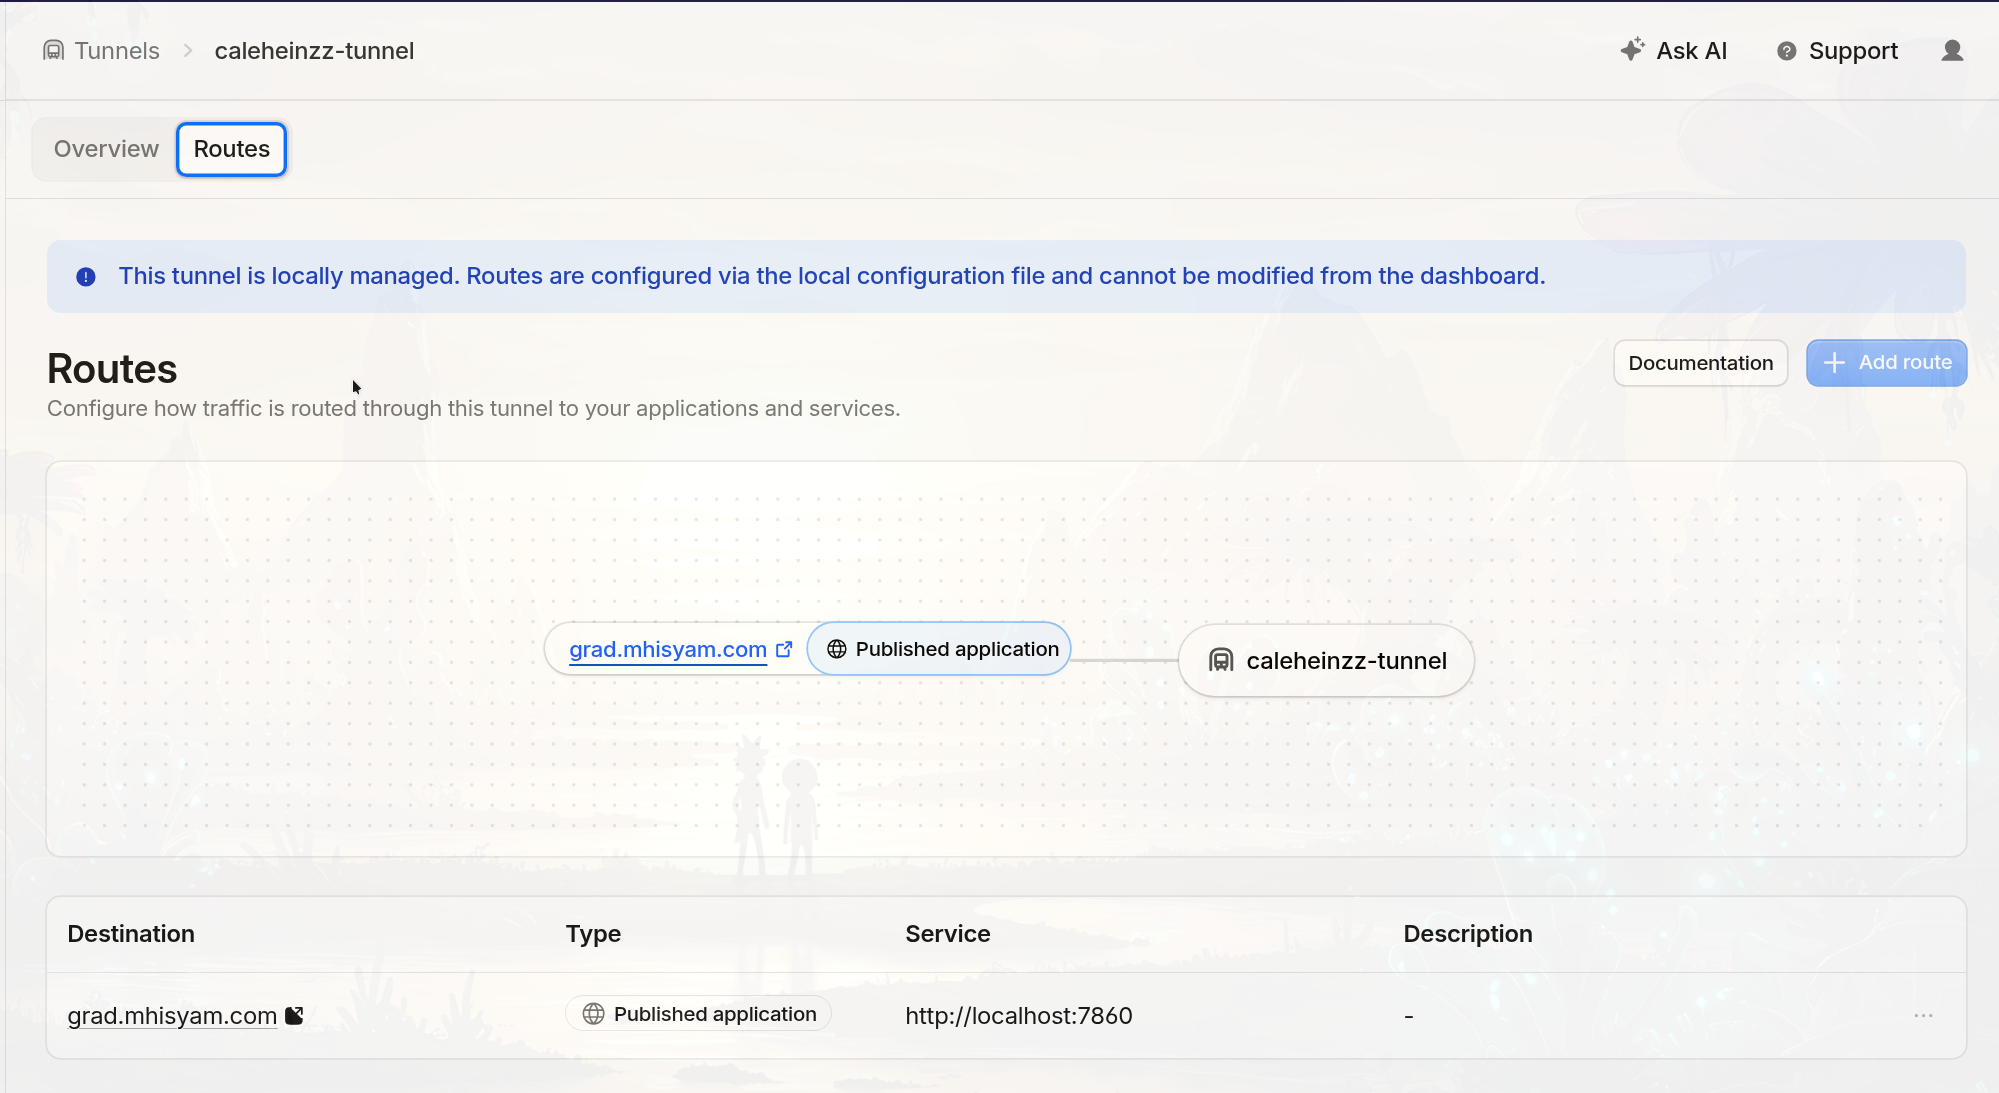
\includegraphics[width=0.78\textwidth]{cloudflare_tunnel}
    \begin{block}{\footnotesize Arsitektur Cloudflare Tunnel}
      \begin{itemize}\tiny
        \item Daemon \texttt{cloudflared} outbound tunnel.
        \item Enkripsi SSL/TLS HTTPS otomatis.
        \item Custom URL: \texttt{https://grad.mhisyam.com}.
      \end{itemize}
    \end{block}
  \end{column}
\end{columns}
\end{frame}

% ─── SLIDE 14: KESIMPULAN ───────────────────────────────────
\begin{frame}{KESIMPULAN PENELITIAN}{Sintesis Capaian Penelitian Berdasarkan Tujuan \& Pengujian}
\begin{block}{\footnotesize Kesimpulan Penelitian (Bab V --- Penutup)}
  \begin{enumerate}\scriptsize
    \item \textbf{Model Terbangun}: Arsitektur U-Net + sCSE + EfficientNet-B3 berhasil dikembangkan. Pada data validasi diperoleh \textbf{Precision 68,68\%}, \textbf{Recall (Sensitivitas) 70,82\%}, dan \textbf{Specificity 97,81\%}. Spesifisitas tinggi membuktikan model sangat jarang salah mengenali paru sehat sebagai pneumonia.
    \item \textbf{Aplikasi Web Gradio}: Prototipe antarmuka web interaktif berhasil dibuat --- menampilkan overlay segmentasi, peta panas Grad-CAM, analisis keparahan (5 tingkat), dan lateralitas infeksi dalam \textbf{1--3 detik}.
    \item \textbf{Dual Lung Masking (PSPNet)}: Meminimalkan bias \textit{shortcut learning} dari teks/penanda DICOM, meningkatkan kepercayaan klinis melalui Grad-CAM \textit{real-time}.
    \item \textbf{Keterbatasan}: Keterbatasan VRAM GPU (8 GB) mengharuskan \textit{gradient accumulation} \& AMP. Resolusi anotasi RSNA yang kasar (\textit{bounding box}) membatasi presisi piksel. Belum ada validasi klinis langsung dengan dokter radiolog.
  \end{enumerate}
\end{block}
\vspace{0.05cm}
\begin{alertblock}{\footnotesize Catatan Penting}
  \scriptsize Sistem ini \textbf{berfungsi sebagai alat bantu skrining awal (triase)}, bukan pengganti keputusan akhir dokter spesialis radiologi.
\end{alertblock}
\end{frame}

% ─── SLIDE 15: SARAN PENGEMBANGAN ───────────────────────────
\begin{frame}{SARAN PENGEMBANGAN}{Rekomendasi untuk Peningkatan Performa \& Penerapan Klinis Masa Depan}
\begin{columns}[T]
  \begin{column}{0.48\textwidth}
    \begin{block}{\footnotesize 1. Rekomendasi Dataset \& Model}
      \begin{itemize}\scriptsize
        \item \textbf{Anotasi Piksel Asli}: Menggunakan dataset rontgen dada dengan anotasi manual \textit{pixel-level} langsung dari dokter spesialis radiologi, menggantikan konversi \textit{bounding box}.
        \item \textbf{Arsitektur Vision Transformer}: Mengeksplorasi ViT-based \textit{segmentation} (\textit{Swin-UNet}, \textit{Medical SAM}) untuk perbandingan kinerja.
      \end{itemize}
    \end{block}
  \end{column}

  \begin{column}{0.48\textwidth}
    \begin{block}{\footnotesize 2. Rekomendasi Klinis \& Sistem}
      \begin{itemize}\scriptsize
        \item \textbf{Validasi Klinis Lokal}: Melakukan uji coba lapangan menggunakan data pasien dari rumah sakit lokal Indonesia untuk menguji generalisasi model terhadap variasi mesin rontgen.
        \item \textbf{Integrasi PACS}: Mengintegrasikan aplikasi web dengan sistem \textit{Picture Archiving and Communication System} (PACS) agar dapat digunakan langsung di lingkungan klinis nyata.
      \end{itemize}
    \end{block}
  \end{column}
\end{columns}
\end{frame}

\end{document}
